\chapter{Introduction générale}

Dans un contexte de transformation numérique des établissements
d\textquotesingle enseignement supérieur au Maroc, la gestion des
processus d\textquotesingle admission et de présélection constitue un
enjeu majeur pour les écoles d\textquotesingle ingénieurs.
L\textquotesingle ENSA Béni Mellal accueille chaque année un nombre
croissant de candidatures pour ses filières d\textquotesingle ingénieur,
tant au niveau Bac+2 qu\textquotesingle au niveau Bac+3.

Le processus actuel de présélection, principalement manuel et basé sur
des fichiers Excel, présente plusieurs limites : risque
d\textquotesingle erreurs humaines, lenteur du traitement, absence de
traçabilité et difficulté de gestion des volumes importants de dossiers.
Le service de la Scolarité a exprimé le besoin d\textquotesingle une
solution informatique capable d\textquotesingle automatiser et de
fiabiliser ce processus.

C\textquotesingle est dans ce contexte que s\textquotesingle inscrit
notre projet de stage : la conception et le développement
d\textquotesingle une plateforme web intelligente de présélection des
candidats. Ce rapport est structuré en quatre chapitres :

\begin{itemize}
\item
  Chapitre 1 --- Contexte du Projet : présentation de
  l\textquotesingle organisme d\textquotesingle accueil, problématique
  et objectifs.
\item
  Chapitre 2 --- Architecture et Base de données : architecture
  Full-Stack, stack technologique et dictionnaire des modèles Django.
\item
  Chapitre 3 --- Logique Métier et Algorithmes : moteur de règles,
  scoring pondéré, pipeline OCR et fuzzy matching.
\item
  Chapitre 4 --- Implémentation, Asynchronisme et Tests : interfaces,
  threading, notifications WebSocket, sécurité et validation.
\end{itemize}

\chapter{Contexte du
Projet}

\section{Introduction}

Ce chapitre présente le cadre général dans lequel
s\textquotesingle inscrit notre stage de fin d\textquotesingle études.
Nous y décrivons l\textquotesingle organisme d\textquotesingle accueil,
le contexte institutionnel, la problématique identifiée et les objectifs
du projet.

\section{Présentation de l\textquotesingle organisme
d\textquotesingle accueil}

\subsection{L\textquotesingle ENSA Béni
Mellal}

L\textquotesingle École Nationale des Sciences Appliquées de Béni Mellal
(ENSA BM) est un établissement public d\textquotesingle enseignement
supérieur rattaché à l\textquotesingle Université Sultan Moulay Slimane
(USMS). Créée en 2003 par décret ministériel n° 2-03-200, elle fait
partie du réseau des douze ENSA marocaines et forme des ingénieurs
d\textquotesingle État dans les domaines des sciences appliquées.

\begin{longtable}[]{@{}
  >{\raggedright\arraybackslash}p{(\columnwidth - 2\tabcolsep) * \real{0.4865}}
  >{\raggedright\arraybackslash}p{(\columnwidth - 2\tabcolsep) * \real{0.4865}}@{}}
\toprule\noalign{}
\caption{Fiche signalétique de l\textquotesingle ENSA BM} \\
\begin{minipage}[b]{\linewidth}\raggedright
\textbf{Rubrique}
\end{minipage} & \begin{minipage}[b]{\linewidth}\raggedright
\textbf{Information}
\end{minipage} \\
\midrule\noalign{}
\endfirsthead
\caption[]{Fiche signalétique de l\textquotesingle ENSA BM (suite)} \\
\begin{minipage}[b]{\linewidth}\raggedright
\textbf{Rubrique}
\end{minipage} & \begin{minipage}[b]{\linewidth}\raggedright
\textbf{Information}
\end{minipage} \\
\midrule\noalign{}
\endhead
\bottomrule\noalign{}
\endlastfoot
Dénomination & École Nationale des Sciences Appliquées de Béni Mellal \\
Sigle & ENSA BM \\
Université & Université Sultan Moulay Slimane (USMS) \\
Statut & Établissement public d\textquotesingle enseignement
supérieur \\
Création & 2003 --- Décret n° 2-03-200 \\
Effectif étudiants & \textasciitilde2 500 (2024-2025) \\
Enseignants & \textasciitilde120 enseignants-chercheurs \\
\end{longtable}

\subsection{Missions et offre de
formation}

L\textquotesingle ENSA BM a pour mission de former des ingénieurs
d\textquotesingle État polyvalents, de développer la recherche
scientifique et l\textquotesingle innovation technologique, et de
contribuer au développement socio-économique de la région Béni
Mellal-Khénifra.

L\textquotesingle école propose quatre filières
d\textquotesingle ingénieur accessibles aux niveaux Bac+2 et Bac+3 :

\begin{longtable}[]{@{}
  >{\raggedright\arraybackslash}p{(\columnwidth - 4\tabcolsep) * \real{0.3243}}
  >{\raggedright\arraybackslash}p{(\columnwidth - 4\tabcolsep) * \real{0.3243}}
  >{\raggedright\arraybackslash}p{(\columnwidth - 4\tabcolsep) * \real{0.3243}}@{}}
\toprule\noalign{}
\caption{Filières d\textquotesingle ingénieur de l\textquotesingle ENSA BM} \\
\begin{minipage}[b]{\linewidth}\raggedright
\textbf{Code}
\end{minipage} & \begin{minipage}[b]{\linewidth}\raggedright
\textbf{Filière}
\end{minipage} & \begin{minipage}[b]{\linewidth}\raggedright
\textbf{Places}
\end{minipage} \\
\midrule\noalign{}
\endfirsthead
\caption[]{Filières d\textquotesingle ingénieur de l\textquotesingle ENSA BM (suite)} \\
\begin{minipage}[b]{\linewidth}\raggedright
\textbf{Code}
\end{minipage} & \begin{minipage}[b]{\linewidth}\raggedright
\textbf{Filière}
\end{minipage} & \begin{minipage}[b]{\linewidth}\raggedright
\textbf{Places}
\end{minipage} \\
\midrule\noalign{}
\endhead
\bottomrule\noalign{}
\endlastfoot
TDI & Télécommunications et Développement Informatique & 30 \\
IACS & Informatique Appliquée et Cybersécurité & 30 \\
IAA & Ingénierie Agro-Alimentaire & 30 \\
G2ER & Génie de l\textquotesingle Énergie et Énergies Renouvelables &
30 \\
\end{longtable}

\subsection{Service de la
Scolarité}

Le service de la Scolarité gère l\textquotesingle ensemble des processus
administratifs liés aux étudiants : inscriptions, examens, stages,
diplomation et présélection des candidats au cycle ingénieur.
C\textquotesingle est le principal bénéficiaire et commanditaire de
notre plateforme.

\section{Contexte et
problématique}

\subsection{Le processus actuel de
présélection}

Le processus actuel de présélection à l\textquotesingle ENSA BM se
déroule en plusieurs étapes manuelles : (1) réception des dossiers
physiques ou par email, (2) vérification manuelle de la conformité des
pièces, (3) saisie des notes dans un fichier Excel, (4) tri et
classement manuel, (5) convocation à l\textquotesingle épreuve écrite,
et (6) saisie des notes d\textquotesingle épreuve et classement final.
Ce processus mobilise plusieurs agents pendant plusieurs semaines.

\subsection{Problèmes
identifiés}

\begin{itemize}
\item
  Traitement lent et chronophage : plusieurs semaines pour quelques
  centaines de dossiers
\item
  Risque élevé d\textquotesingle erreurs de saisie lors de la
  transcription manuelle des notes
\item
  Absence totale de traçabilité des décisions prises
\item
  Manque de transparence : les candidats n\textquotesingle ont aucune
  visibilité sur l\textquotesingle état de leur dossier
\item
  Doublons non détectés : difficulté d\textquotesingle identifier les
  candidatures multiples
\item
  Classement approximatif : calculs manuels sujets à erreur
\end{itemize}

\subsection{Le système LMD
marocain}

Le système LMD marocain structure les études supérieures en trois
cycles. Chaque semestre est évalué sur 20 points. Les mentions sont
attribuées selon les seuils suivants :

\begin{longtable}[]{@{}
  >{\raggedright\arraybackslash}p{(\columnwidth - 2\tabcolsep) * \real{0.4865}}
  >{\raggedright\arraybackslash}p{(\columnwidth - 2\tabcolsep) * \real{0.4865}}@{}}
\toprule\noalign{}
\begin{minipage}[b]{\linewidth}\raggedright
\textbf{Moyenne}
\end{minipage} & \begin{minipage}[b]{\linewidth}\raggedright
\textbf{Mention}
\end{minipage} \\
\midrule\noalign{}
\endhead
\bottomrule\noalign{}
\endlastfoot
$\geq$ 16.00 & Très Bien \\
$\geq$ 14.00 & Bien \\
$\geq$ 12.00 & Assez Bien \\
$\geq$ 10.00 & Passable \\
\end{longtable}

Notre plateforme doit impérativement respecter ces seuils pour le calcul
automatique des mentions et du scoring académique.

\section{Objectifs du projet}

\subsection{Objectif principal}

Concevoir et développer une plateforme web complète permettant
d\textquotesingle automatiser et de fiabiliser le processus de
présélection des candidats aux filières d\textquotesingle ingénieur de
l\textquotesingle ENSA BM.

\subsection{Objectifs
spécifiques}

\begin{itemize}
\item
  Automatisation du rejet des dossiers non conformes via un moteur de
  règles configurable
\item
  Scoring académique pondéré par filière avec fuzzy matching des
  matières
\item
  Classement automatique des candidats intégrant dossier (40\%) et
  épreuve écrite (60\%)
\item
  Notifications en temps réel via WebSocket et email SMTP
\item
  Traçabilité et audit complet du processus de présélection
\item
  Import des notes d\textquotesingle épreuve écrite au format Excel
\end{itemize}

\section{Périmètre fonctionnel}

\begin{longtable}[]{@{}
  >{\raggedright\arraybackslash}p{(\columnwidth - 2\tabcolsep) * \real{0.4865}}
  >{\raggedright\arraybackslash}p{(\columnwidth - 2\tabcolsep) * \real{0.4865}}@{}}
\toprule\noalign{}
\caption{Périmètre fonctionnel du projet} \\
\begin{minipage}[b]{\linewidth}\raggedright
\textbf{Fonctionnalité}
\end{minipage} & \begin{minipage}[b]{\linewidth}\raggedright
\textbf{Inclus}
\end{minipage} \\
\midrule\noalign{}
\endfirsthead
\caption[]{Périmètre fonctionnel du projet (suite)} \\
\begin{minipage}[b]{\linewidth}\raggedright
\textbf{Fonctionnalité}
\end{minipage} & \begin{minipage}[b]{\linewidth}\raggedright
\textbf{Inclus}
\end{minipage} \\
\midrule\noalign{}
\endhead
\bottomrule\noalign{}
\endlastfoot
Inscription et authentification JWT & Oui \\
Dépôt de dossier multi-étapes & Oui \\
Moteur de règles de rejet automatique & Oui \\
Scoring pondéré par filière & Oui \\
Dashboard responsable avec KPIs & Oui \\
Import notes Excel & Oui \\
Notifications WebSocket + SMTP & Oui \\
Export résultats Excel & Oui \\
Application mobile native & Non (hors scope) \\
Intégration Massar & Non (hors scope) \\
\end{longtable}

\section{Méthodologie de travail}

Nous avons adopté une approche agile itérative, organisée en sprints
hebdomadaires sur 4 semaines. Chaque sprint produit un incrément
fonctionnel testé et validé.

\begin{longtable}[]{@{}
  >{\raggedright\arraybackslash}p{(\columnwidth - 4\tabcolsep) * \real{0.3243}}
  >{\raggedright\arraybackslash}p{(\columnwidth - 4\tabcolsep) * \real{0.3243}}
  >{\raggedright\arraybackslash}p{(\columnwidth - 4\tabcolsep) * \real{0.3243}}@{}}
\toprule\noalign{}
\caption{Planning prévisionnel du projet} \\
\begin{minipage}[b]{\linewidth}\raggedright
\textbf{Semaine}
\end{minipage} & \begin{minipage}[b]{\linewidth}\raggedright
\textbf{Phase}
\end{minipage} & \begin{minipage}[b]{\linewidth}\raggedright
\textbf{Livrables}
\end{minipage} \\
\midrule\noalign{}
\endfirsthead
\caption[]{Planning prévisionnel du projet (suite)} \\
\begin{minipage}[b]{\linewidth}\raggedright
\textbf{Semaine}
\end{minipage} & \begin{minipage}[b]{\linewidth}\raggedright
\textbf{Phase}
\end{minipage} & \begin{minipage}[b]{\linewidth}\raggedright
\textbf{Livrables}
\end{minipage} \\
\midrule\noalign{}
\endhead
\bottomrule\noalign{}
\endlastfoot
S1 & Fondations Backend & Modèles Django, API REST, Auth JWT \\
S2 & Intelligence métier & Moteur de règles, Scoring, OCR \\
S3 & Frontend React & Pages candidat, Dashboard, Formulaires \\
S4 & Tests et finalisation & Tests, Corrections, Documentation \\
\end{longtable}

\section{Conclusion}

Ce chapitre a permis de situer le cadre institutionnel de notre stage et
de définir clairement la problématique et les objectifs du projet. Le
chapitre suivant présentera l\textquotesingle architecture technique et
le modèle de données de la plateforme.

\chapter{Architecture et Base de
données}

\section{Introduction}

Ce chapitre détaille l\textquotesingle architecture technique de la
plateforme, le choix des technologies, l\textquotesingle organisation
modulaire du code et le dictionnaire complet des modèles Django.

\begin{figure}[htbp]
\centering
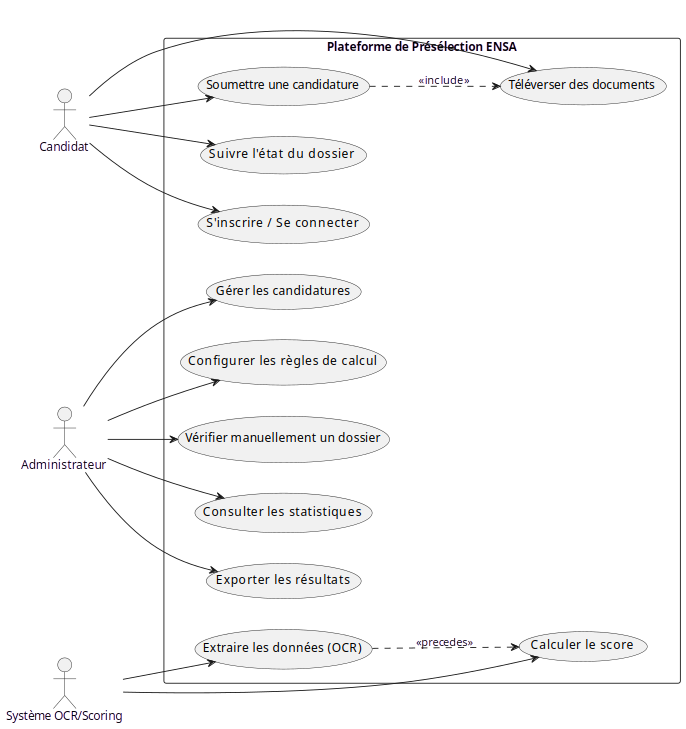
\includegraphics[width=6.18264in,height=6.79722in]{media/image3.png}
\end{figure}

\section{Architecture globale}

\subsection{Vue d\textquotesingle ensemble}

L\textquotesingle application repose sur une architecture moderne
Full-Stack Client-Serveur à trois niveaux :

\begin{itemize}
\item
  Frontend : React 18 compilé via Vite, avec Tailwind CSS pour le rendu
  responsive. L\textquotesingle architecture s\textquotesingle appuie
  sur des composants réutilisables, React Router v6 et un state
  management optimisé via Context API.
\item
  Backend : Django 4.2 LTS et Django REST Framework (DRF), exposant une
  API REST sécurisée par JWT (SimpleJWT). Le backend est organisé en 5
  applications Django indépendantes.
\item
  Base de données : PostgreSQL 15 géré par l\textquotesingle ORM Django,
  assurant la persistance des candidatures, configurations et
  historiques.
\item
  Temps réel : Django Channels 4.0 avec Redis comme channel layer pour
  les WebSockets (notifications en temps réel avec barre de
  progression).

  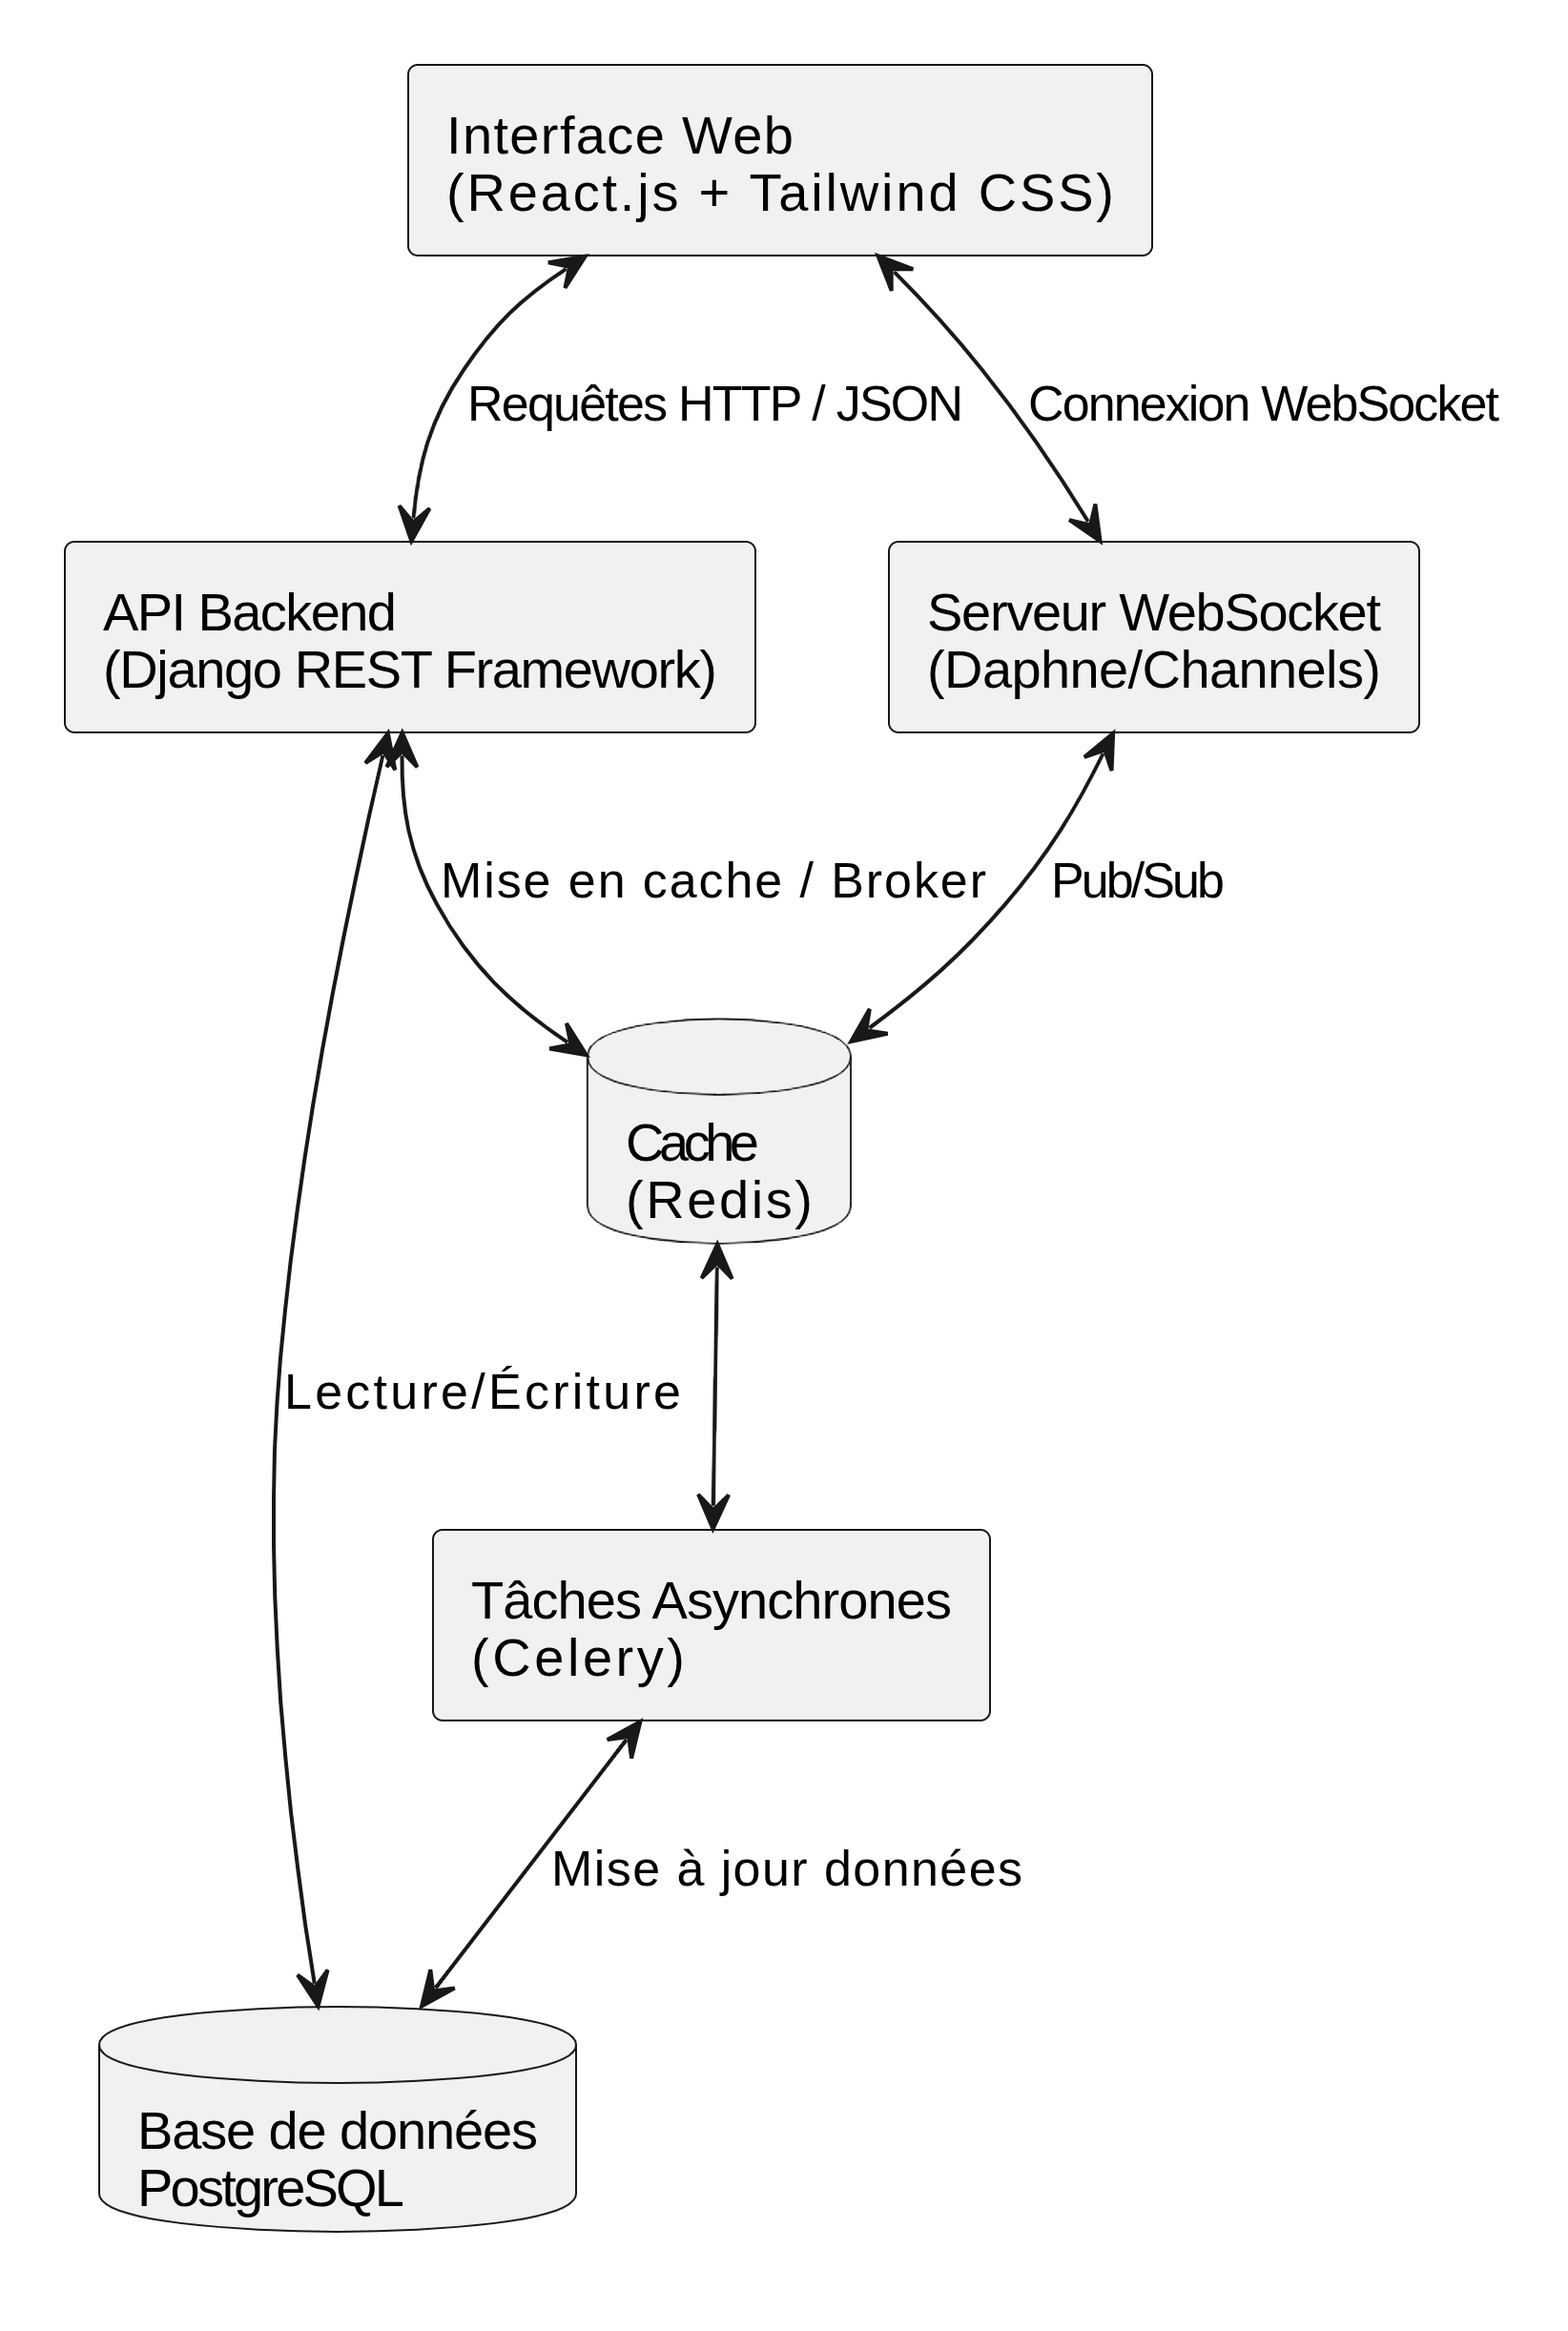
\includegraphics[width=2.81319in,height=4.18125in]{media/image5.png}
\end{itemize}

\subsection{Architecture REST
stateless}

Le frontend communique avec le backend exclusivement via des endpoints
REST sécurisés par JWT. Les réponses sont au format JSON. Le pattern est
strictement stateless côté serveur, à l\textquotesingle exception des
connexions WebSocket persistantes pour les notifications.

\section{Stack technologique}

\begin{longtable}[]{@{}
  >{\raggedright\arraybackslash}p{(\columnwidth - 4\tabcolsep) * \real{0.3243}}
  >{\raggedright\arraybackslash}p{(\columnwidth - 4\tabcolsep) * \real{0.3243}}
  >{\raggedright\arraybackslash}p{(\columnwidth - 4\tabcolsep) * \real{0.3243}}@{}}
\toprule\noalign{}
\caption{Stack technologique du projet} \\
\begin{minipage}[b]{\linewidth}\raggedright
\textbf{Technologie}
\end{minipage} & \begin{minipage}[b]{\linewidth}\raggedright
\textbf{Version}
\end{minipage} & \begin{minipage}[b]{\linewidth}\raggedright
\textbf{Rôle}
\end{minipage} \\
\midrule\noalign{}
\endfirsthead
\caption[]{Stack technologique du projet (suite)} \\
\begin{minipage}[b]{\linewidth}\raggedright
\textbf{Technologie}
\end{minipage} & \begin{minipage}[b]{\linewidth}\raggedright
\textbf{Version}
\end{minipage} & \begin{minipage}[b]{\linewidth}\raggedright
\textbf{Rôle}
\end{minipage} \\
\midrule\noalign{}
\endhead
\bottomrule\noalign{}
\endlastfoot
Django & 4.2 LTS & Framework backend principal \\
Django REST Framework & 3.17 & Construction de l\textquotesingle API
REST \\
Django Channels & 4.0 & WebSockets temps réel \\
SimpleJWT & 5.5 & Authentification par tokens JWT \\
React & 18 & Framework frontend SPA \\
Tailwind CSS & 3.x & Framework CSS utilitaire \\
PostgreSQL & 15 & Base de données relationnelle \\
Redis & 7.x & Channel Layer WebSocket \\
pdfplumber + pytesseract & --- & Extraction OCR \\
fuzzywuzzy & 0.18 & Correspondance floue des matières \\
openpyxl & --- & Import/Export Excel \\
\end{longtable}

\section{Organisation modulaire du
backend}

Le backend est structuré en 5 applications Django indépendantes, chacune
gérant un domaine métier spécifique :

\begin{longtable}[]{@{}
  >{\raggedright\arraybackslash}p{(\columnwidth - 4\tabcolsep) * \real{0.3243}}
  >{\raggedright\arraybackslash}p{(\columnwidth - 4\tabcolsep) * \real{0.3243}}
  >{\raggedright\arraybackslash}p{(\columnwidth - 4\tabcolsep) * \real{0.3243}}@{}}
\toprule\noalign{}
\caption{Applications Django du backend} \\
\begin{minipage}[b]{\linewidth}\raggedright
\textbf{Application}
\end{minipage} & \begin{minipage}[b]{\linewidth}\raggedright
\textbf{Responsabilité}
\end{minipage} & \begin{minipage}[b]{\linewidth}\raggedright
\textbf{Fichiers clés}
\end{minipage} \\
\midrule\noalign{}
\endfirsthead
\caption[]{Applications Django du backend (suite)} \\
\begin{minipage}[b]{\linewidth}\raggedright
\textbf{Application}
\end{minipage} & \begin{minipage}[b]{\linewidth}\raggedright
\textbf{Responsabilité}
\end{minipage} & \begin{minipage}[b]{\linewidth}\raggedright
\textbf{Fichiers clés}
\end{minipage} \\
\midrule\noalign{}
\endhead
\bottomrule\noalign{}
\endlastfoot
users & Authentification, comptes, profils candidats & models.py,
serializers.py, views.py \\
candidatures & Dossiers, documents, notes, services métier & models.py,
views.py, services/ \\
administration & Filières, diplômes, épreuves, historique & models.py,
views.py \\
scoring & Règles de rejet, configuration scoring & models.py,
views.py \\
notifications & Notifications email et WebSocket & models.py,
consumers.py, views.py \\
\end{longtable}

Le répertoire candidatures/services/ contient la logique métier critique
:

\begin{longtable}[]{@{}
  >{\raggedright\arraybackslash}p{(\columnwidth - 4\tabcolsep) * \real{0.3117}}
  >{\raggedright\arraybackslash}p{(\columnwidth - 4\tabcolsep) * \real{0.3506}}
  >{\raggedright\arraybackslash}p{(\columnwidth - 4\tabcolsep) * \real{0.3117}}@{}}
\toprule\noalign{}
\caption{Services métier du module candidatures} \\
\begin{minipage}[b]{\linewidth}\raggedright
\textbf{Service}
\end{minipage} & \begin{minipage}[b]{\linewidth}\raggedright
\textbf{Fichier}
\end{minipage} & \begin{minipage}[b]{\linewidth}\raggedright
\textbf{Rôle}
\end{minipage} \\
\midrule\noalign{}
\endfirsthead
\caption[]{Services métier du module candidatures (suite)} \\
\begin{minipage}[b]{\linewidth}\raggedright
\textbf{Service}
\end{minipage} & \begin{minipage}[b]{\linewidth}\raggedright
\textbf{Fichier}
\end{minipage} & \begin{minipage}[b]{\linewidth}\raggedright
\textbf{Rôle}
\end{minipage} \\
\midrule\noalign{}
\endhead
\bottomrule\noalign{}
\endlastfoot
Extraction OCR & extraction.py & Extraction des informations depuis les
documents scannés \\
Fuzzy Matching & fuzzy\_matching.py & Correspondance floue des noms de
matières \\
Règles de rejet & regles.py & Application des 7 types de règles de rejet
automatique \\
Scoring & scoring.py & Calcul du score pondéré par filière \\
Vérification & verification\_document.py & Vérification
d\textquotesingle authenticité des documents \\
Invitation PDF & invitation\_pdf.py & Génération des convocations au
format PDF \\
\end{longtable}

\begin{figure}[htbp]
\centering
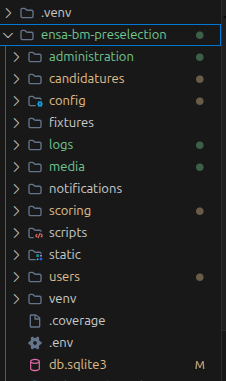
\includegraphics[width=2.35417in,height=3.96875in]{media/image6.png}
\end{figure}

\section{Dictionnaire des modèles
Django}

Le modèle relationnel est structuré autour de 12 entités principales
réparties dans les applications Django. Nous détaillons ci-dessous
chaque modèle.

\subsection{Application Users}

Le modèle User étend AbstractBaseUser de Django pour personnaliser
l\textquotesingle authentification. L\textquotesingle identification se
fait par email et CIN (Carte d\textquotesingle Identité Nationale).
Trois rôles sont définis : CANDIDAT, RESPONSABLE et ADMIN, implémentant
un contrôle d\textquotesingle accès RBAC.

\begin{longtable}[]{@{}
  >{\raggedright\arraybackslash}p{(\columnwidth - 4\tabcolsep) * \real{0.3243}}
  >{\raggedright\arraybackslash}p{(\columnwidth - 4\tabcolsep) * \real{0.3243}}
  >{\raggedright\arraybackslash}p{(\columnwidth - 4\tabcolsep) * \real{0.3243}}@{}}
\toprule\noalign{}
\begin{minipage}[b]{\linewidth}\raggedright
\textbf{Attribut}
\end{minipage} & \begin{minipage}[b]{\linewidth}\raggedright
\textbf{Type}
\end{minipage} & \begin{minipage}[b]{\linewidth}\raggedright
\textbf{Contrainte}
\end{minipage} \\
\midrule\noalign{}
\endhead
\bottomrule\noalign{}
\endlastfoot
id & UUID & Clé primaire auto-générée \\
email & VARCHAR & UNIQUE, NOT NULL \\
cin & VARCHAR & UNIQUE, NOT NULL \\
role & ENUM & CANDIDAT / RESPONSABLE / ADMIN \\
is\_active & BOOLEAN & Défaut : True \\
password & VARCHAR & Hashé via PBKDF2 \\
\end{longtable}

Le modèle Candidat est relié en OneToOne à User et stocke le profil
détaillé :

\begin{longtable}[]{@{}
  >{\raggedright\arraybackslash}p{(\columnwidth - 4\tabcolsep) * \real{0.3243}}
  >{\raggedright\arraybackslash}p{(\columnwidth - 4\tabcolsep) * \real{0.3243}}
  >{\raggedright\arraybackslash}p{(\columnwidth - 4\tabcolsep) * \real{0.3243}}@{}}
\toprule\noalign{}
\begin{minipage}[b]{\linewidth}\raggedright
\textbf{Attribut}
\end{minipage} & \begin{minipage}[b]{\linewidth}\raggedright
\textbf{Type}
\end{minipage} & \begin{minipage}[b]{\linewidth}\raggedright
\textbf{Contrainte}
\end{minipage} \\
\midrule\noalign{}
\endhead
\bottomrule\noalign{}
\endlastfoot
id & UUID & Clé primaire \\
user\_id & FK → User & OneToOne, CASCADE \\
nom & VARCHAR & NOT NULL \\
prenom & VARCHAR & NOT NULL \\
telephone & VARCHAR & Optionnel \\
date\_naissance & DATE & NOT NULL \\
\end{longtable}

\subsection{Application
Candidatures}

Le modèle Dossier est le modèle central de
l\textquotesingle application. Il lie un Candidat à une Filière et
contient le statut, les scores calculés et les motifs de rejet
éventuels.

\begin{longtable}[]{@{}
  >{\raggedright\arraybackslash}p{(\columnwidth - 4\tabcolsep) * \real{0.3243}}
  >{\raggedright\arraybackslash}p{(\columnwidth - 4\tabcolsep) * \real{0.3243}}
  >{\raggedright\arraybackslash}p{(\columnwidth - 4\tabcolsep) * \real{0.3243}}@{}}
\toprule\noalign{}
\begin{minipage}[b]{\linewidth}\raggedright
\textbf{Attribut}
\end{minipage} & \begin{minipage}[b]{\linewidth}\raggedright
\textbf{Type}
\end{minipage} & \begin{minipage}[b]{\linewidth}\raggedright
\textbf{Contrainte}
\end{minipage} \\
\midrule\noalign{}
\endhead
\bottomrule\noalign{}
\endlastfoot
id & UUID & Clé primaire \\
candidat\_id & FK → Candidat & CASCADE \\
filiere\_id & FK → Filiere & CASCADE \\
statut & ENUM & 11 valeurs possibles \\
score & DECIMAL & Score dossier calculé \\
score\_final & DECIMAL & 40\% dossier + 60\% épreuve \\
rang\_final & INT & Classement par filière \\
mention & ENUM & Auto-calculé \\
moyenne\_generale & DECIMAL & Moyenne des semestres \\
\end{longtable}

Le modèle Document gère les pièces justificatives uploadées par le
candidat :

\begin{longtable}[]{@{}
  >{\raggedright\arraybackslash}p{(\columnwidth - 4\tabcolsep) * \real{0.3200}}
  >{\raggedright\arraybackslash}p{(\columnwidth - 4\tabcolsep) * \real{0.3200}}
  >{\raggedright\arraybackslash}p{(\columnwidth - 4\tabcolsep) * \real{0.3333}}@{}}
\toprule\noalign{}
\begin{minipage}[b]{\linewidth}\raggedright
\textbf{Attribut}
\end{minipage} & \begin{minipage}[b]{\linewidth}\raggedright
\textbf{Type}
\end{minipage} & \begin{minipage}[b]{\linewidth}\raggedright
\textbf{Contrainte}
\end{minipage} \\
\midrule\noalign{}
\endhead
\bottomrule\noalign{}
\endlastfoot
id & UUID & Clé primaire \\
dossier\_id & FK → Dossier & CASCADE \\
type\_doc & ENUM & DIPLOME / RELEVE / CIN / PHOTO \\
fichier & FILE & Stocké dans media/dossiers/\{uuid\}/ \\
qualite\_ocr & DECIMAL & Score de confiance OCR \\
\end{longtable}

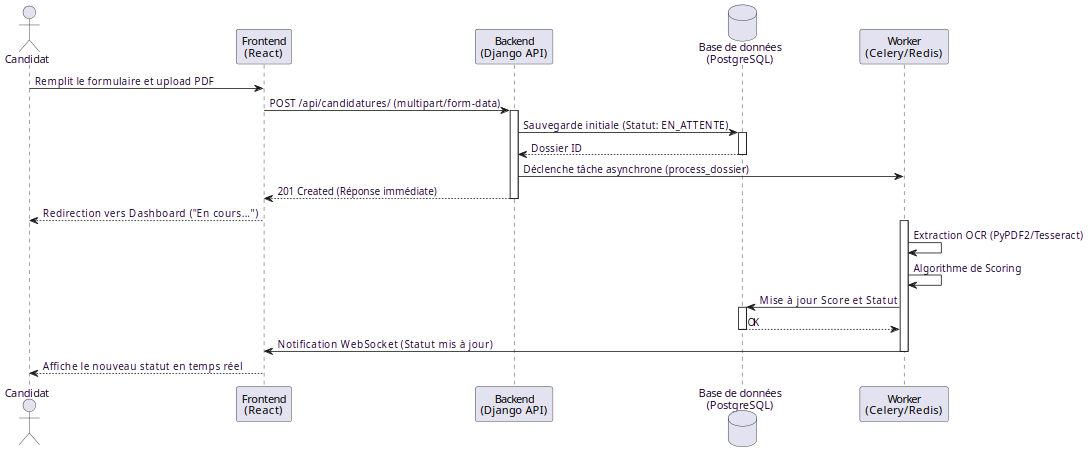
\includegraphics[width=7.84653in,height=3.66875in]{media/image7.png}
modèle NoteSemestre remplace l\textquotesingle ancienne approche par
NoteMatiere. Il intègre la moyenne par semestre, la session et la
mention calculée dynamiquement :

\begin{longtable}[]{@{}
  >{\raggedright\arraybackslash}p{(\columnwidth - 4\tabcolsep) * \real{0.3243}}
  >{\raggedright\arraybackslash}p{(\columnwidth - 4\tabcolsep) * \real{0.3243}}
  >{\raggedright\arraybackslash}p{(\columnwidth - 4\tabcolsep) * \real{0.3243}}@{}}
\toprule\noalign{}
\begin{minipage}[b]{\linewidth}\raggedright
\textbf{Attribut}
\end{minipage} & \begin{minipage}[b]{\linewidth}\raggedright
\textbf{Type}
\end{minipage} & \begin{minipage}[b]{\linewidth}\raggedright
\textbf{Contrainte}
\end{minipage} \\
\midrule\noalign{}
\endhead
\bottomrule\noalign{}
\endlastfoot
id & UUID & Clé primaire \\
dossier\_id & FK → Dossier & CASCADE \\
semestre & ENUM & S1 à S6 \\
moyenne & DECIMAL & Plage stricte {[}10.00, 20.00{]} \\
session & ENUM & NORMALE / RATTRAPAGE \\
mention & ENUM & Auto-calculé (editable=False) \\
\end{longtable}

\subsection{Application Administration et
Scoring}

Le modèle Filiere définit les filières du cycle ingénieur avec leurs
paramètres :

\begin{longtable}[]{@{}
  >{\raggedright\arraybackslash}p{(\columnwidth - 4\tabcolsep) * \real{0.3243}}
  >{\raggedright\arraybackslash}p{(\columnwidth - 4\tabcolsep) * \real{0.3243}}
  >{\raggedright\arraybackslash}p{(\columnwidth - 4\tabcolsep) * \real{0.3243}}@{}}
\toprule\noalign{}
\begin{minipage}[b]{\linewidth}\raggedright
\textbf{Attribut}
\end{minipage} & \begin{minipage}[b]{\linewidth}\raggedright
\textbf{Type}
\end{minipage} & \begin{minipage}[b]{\linewidth}\raggedright
\textbf{Contrainte}
\end{minipage} \\
\midrule\noalign{}
\endhead
\bottomrule\noalign{}
\endlastfoot
id & UUID & Clé primaire \\
nom & VARCHAR & NOT NULL \\
code & VARCHAR & UNIQUE (TDI, IACS, IAA, G2ER) \\
niveau & ENUM & BAC2 / BAC3 \\
places\_disponibles & INT & Défaut : 30 \\
\end{longtable}

Les modèles EpreuveEcrite et NoteEcrite gèrent la logistique du concours
écrit :

\begin{longtable}[]{@{}
  >{\raggedright\arraybackslash}p{(\columnwidth - 4\tabcolsep) * \real{0.3243}}
  >{\raggedright\arraybackslash}p{(\columnwidth - 4\tabcolsep) * \real{0.3243}}
  >{\raggedright\arraybackslash}p{(\columnwidth - 4\tabcolsep) * \real{0.3243}}@{}}
\toprule\noalign{}
\caption{Modèles d\textquotesingle administration et scoring} \\
\begin{minipage}[b]{\linewidth}\raggedright
\textbf{Modèle}
\end{minipage} & \begin{minipage}[b]{\linewidth}\raggedright
\textbf{Attributs clés}
\end{minipage} & \begin{minipage}[b]{\linewidth}\raggedright
\textbf{Rôle}
\end{minipage} \\
\midrule\noalign{}
\endfirsthead
\caption[]{Modèles d\textquotesingle administration et scoring (suite)} \\
\begin{minipage}[b]{\linewidth}\raggedright
\textbf{Modèle}
\end{minipage} & \begin{minipage}[b]{\linewidth}\raggedright
\textbf{Attributs clés}
\end{minipage} & \begin{minipage}[b]{\linewidth}\raggedright
\textbf{Rôle}
\end{minipage} \\
\midrule\noalign{}
\endhead
\bottomrule\noalign{}
\endlastfoot
EpreuveEcrite & nom, date\_epreuve, seuil\_admission, statut & Gestion
de l\textquotesingle épreuve par filière \\
NoteEcrite & note, resultat, rang\_final & Note individuelle et
classement \\
ConfigScoring & matiere, poids, bonus\_mention & Pondération scoring par
filière \\
RegleRejet & type\_regle, parametre, is\_active, message & Règle de
rejet configurable \\
HistoriqueAction & action, commentaire, timestamp & Traçabilité des
décisions \\
\end{longtable}

\section{Relations et
cardinalités}

\begin{longtable}[]{@{}
  >{\raggedright\arraybackslash}p{(\columnwidth - 4\tabcolsep) * \real{0.3243}}
  >{\raggedright\arraybackslash}p{(\columnwidth - 4\tabcolsep) * \real{0.3243}}
  >{\raggedright\arraybackslash}p{(\columnwidth - 4\tabcolsep) * \real{0.3243}}@{}}
\toprule\noalign{}
\caption{Relations et cardinalités du modèle de données} \\
\begin{minipage}[b]{\linewidth}\raggedright
\textbf{Relation}
\end{minipage} & \begin{minipage}[b]{\linewidth}\raggedright
\textbf{Type}
\end{minipage} & \begin{minipage}[b]{\linewidth}\raggedright
\textbf{Cardinalité}
\end{minipage} \\
\midrule\noalign{}
\endfirsthead
\caption[]{Relations et cardinalités du modèle de données (suite)} \\
\begin{minipage}[b]{\linewidth}\raggedright
\textbf{Relation}
\end{minipage} & \begin{minipage}[b]{\linewidth}\raggedright
\textbf{Type}
\end{minipage} & \begin{minipage}[b]{\linewidth}\raggedright
\textbf{Cardinalité}
\end{minipage} \\
\midrule\noalign{}
\endhead
\bottomrule\noalign{}
\endlastfoot
User → Candidat & OneToOne & 1..1 \\
Candidat → Dossier & OneToMany & 1..* \\
Dossier → Document & OneToMany & 1..4 \\
Dossier → NoteSemestre & OneToMany & 1..6 \\
Filiere → Dossier & OneToMany & 1..* \\
Filiere → RegleRejet & OneToMany & 1..* \\
Filiere → EpreuveEcrite & OneToMany & 1..* \\
EpreuveEcrite → NoteEcrite & OneToMany & 1..* \\
Dossier → HistoriqueAction & OneToMany & 1..* \\
User → Notification & OneToMany & 1..* \\
\end{longtable}

\section{Machine d\textquotesingle états du
dossier}

Le dossier suit une machine d\textquotesingle états stricte implémentée
dans la méthode changer\_statut() du modèle. Chaque transition crée
automatiquement un enregistrement HistoriqueAction pour la traçabilité :

\begin{longtable}[]{@{}
  >{\raggedright\arraybackslash}p{(\columnwidth - 2\tabcolsep) * \real{0.4865}}
  >{\raggedright\arraybackslash}p{(\columnwidth - 2\tabcolsep) * \real{0.4865}}@{}}
\toprule\noalign{}
\caption{Tableau 2.6 : Machine d\textquotesingle états du dossier de candidature} \\
\begin{minipage}[b]{\linewidth}\raggedright
\textbf{État}
\end{minipage} & \begin{minipage}[b]{\linewidth}\raggedright
\textbf{Transitions possibles}
\end{minipage} \\
\midrule\noalign{}
\endfirsthead
\caption[]{Tableau 2.6 : Machine d\textquotesingle états du dossier de candidature (suite)} \\
\begin{minipage}[b]{\linewidth}\raggedright
\textbf{État}
\end{minipage} & \begin{minipage}[b]{\linewidth}\raggedright
\textbf{Transitions possibles}
\end{minipage} \\
\midrule\noalign{}
\endhead
\bottomrule\noalign{}
\endlastfoot
BROUILLON & → EN\_TRAITEMENT (soumission) \\
EN\_TRAITEMENT & → REJETE\_AUTO \textbar{} EN\_ATTENTE \textbar{}
INCOMPLET \textbar{} SUSPECT \\
INCOMPLET & → EN\_TRAITEMENT (complétion) \\
SUSPECT & → EN\_ATTENTE \textbar{} REJETE\_FINAL (décision manuelle) \\
EN\_ATTENTE & → PRESELECTIONNE \textbar{} REJETE\_FINAL \\
PRESELECTIONNE & → ADMIS\_FINAL \textbar{} RECALE\_FINAL \textbar{}
ABSENT\_ECRIT \\
\end{longtable}

\begin{figure}[htbp]
\centering
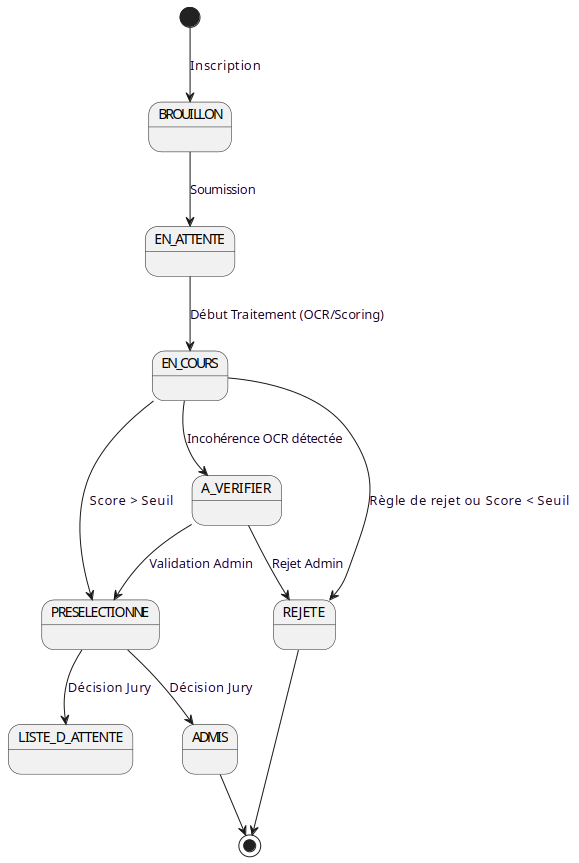
\includegraphics[width=4.29236in,height=6.62847in]{media/image9.png}
\end{figure}

\section{Conclusion}

Ce chapitre a détaillé l\textquotesingle architecture Full-Stack de la
plateforme et le modèle de données relationnel complet.
L\textquotesingle organisation modulaire en 5 applications Django assure
une séparation claire des responsabilités. Le chapitre suivant
présentera la logique métier et les algorithmes de scoring et
d\textquotesingle OCR.

\chapter{Logique Métier et
Algorithmes}

\section{Introduction}

Ce chapitre expose en détail les algorithmes et la logique métier qui
constituent le cœur intelligent de la plateforme. Nous y décrivons le
moteur de règles de rejet, l\textquotesingle algorithme de scoring
pondéré par filière, le pipeline OCR avec fuzzy matching, et les
formules mathématiques appliquées.

\section{Moteur de règles de rejet
automatique}

\subsection{Principe de
fonctionnement}

Le moteur de règles applique séquentiellement un ensemble de
vérifications configurables par filière. Dès qu\textquotesingle une
règle est violée, le dossier est automatiquement rejeté avec le motif
correspondant (pattern court-circuit). Chaque règle peut être activée ou
désactivée individuellement par l\textquotesingle administrateur.

\subsection{Types de règles
implémentés}

\begin{longtable}[]{@{}
  >{\raggedright\arraybackslash}p{(\columnwidth - 4\tabcolsep) * \real{0.3333}}
  >{\raggedright\arraybackslash}p{(\columnwidth - 4\tabcolsep) * \real{0.3200}}
  >{\raggedright\arraybackslash}p{(\columnwidth - 4\tabcolsep) * \real{0.3200}}@{}}
\toprule\noalign{}
\caption{Les 7 types de règles de rejet automatique} \\
\begin{minipage}[b]{\linewidth}\raggedright
\textbf{Code Règle}
\end{minipage} & \begin{minipage}[b]{\linewidth}\raggedright
\textbf{Description}
\end{minipage} & \begin{minipage}[b]{\linewidth}\raggedright
\textbf{Paramètre}
\end{minipage} \\
\midrule\noalign{}
\endfirsthead
\caption[]{Les 7 types de règles de rejet automatique (suite)} \\
\begin{minipage}[b]{\linewidth}\raggedright
\textbf{Code Règle}
\end{minipage} & \begin{minipage}[b]{\linewidth}\raggedright
\textbf{Description}
\end{minipage} & \begin{minipage}[b]{\linewidth}\raggedright
\textbf{Paramètre}
\end{minipage} \\
\midrule\noalign{}
\endhead
\bottomrule\noalign{}
\endlastfoot
DIPLOME\_INVALIDE & Diplôme non accepté pour la filière cible & Liste
des diplômes autorisés \\
MOYENNE\_INSUFFISANTE & Moyenne générale en dessous du seuil minimal &
Seuil minimal (ex: 10.00) \\
NOTE\_ELIMINATOIRE & Note éliminatoire dans une matière clé & Seuil et
matière \\
DOUBLON\_CIN & CIN déjà utilisé dans un autre dossier actif &
Automatique \\
DOCUMENT\_MANQUANT & Document obligatoire absent du dossier & Liste des
types requis \\
DATE\_INCOHERENTE & Incohérence dans les dates du diplôme &
Automatique \\
ETABLISSEMENT\_INVALIDE & Établissement d\textquotesingle origine non
reconnu & Liste blanche \\
\end{longtable}

\begin{figure}[htbp]
\centering
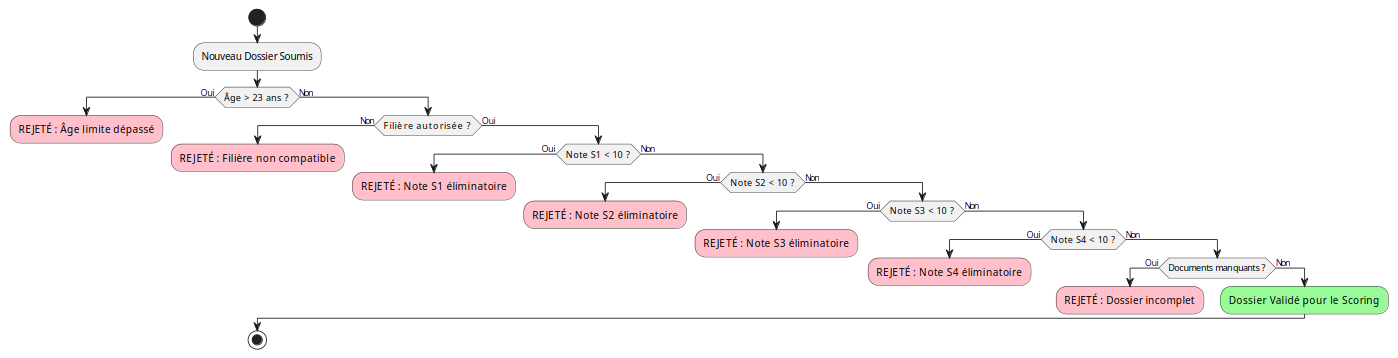
\includegraphics[width=7.12153in,height=1.84861in]{media/image11.png}
\end{figure}

\subsection{Journalisation des
rejets}

Chaque rejet automatique génère un enregistrement HistoriqueAction
contenant le motif précis de rejet, la règle déclenchée et
l\textquotesingle horodatage. Le statut du dossier passe à REJETE\_AUTO
et le candidat est notifié automatiquement par email.

\section{Algorithme de scoring pondéré par
filière}

\subsection{Principe général}

Le scoring repose sur une pondération configurable par filière. Chaque
filière définit des coefficients par catégorie de matières. Les moyennes
semestrielles du candidat sont regroupées par catégorie via le fuzzy
matching, puis pondérées selon les coefficients de la filière cible.

\subsection{Coefficients des quatre
filières}

Le moteur de scoring applique les pondérations suivantes sur les
catégories de matières extraites, en fonction de la filière choisie par
le candidat :

\begin{longtable}[]{@{}
  >{\raggedright\arraybackslash}p{(\columnwidth - 12\tabcolsep) * \real{0.1373}}
  >{\raggedright\arraybackslash}p{(\columnwidth - 12\tabcolsep) * \real{0.1078}}
  >{\raggedright\arraybackslash}p{(\columnwidth - 12\tabcolsep) * \real{0.1078}}
  >{\raggedright\arraybackslash}p{(\columnwidth - 12\tabcolsep) * \real{0.1569}}
  >{\raggedright\arraybackslash}p{(\columnwidth - 12\tabcolsep) * \real{0.1667}}
  >{\raggedright\arraybackslash}p{(\columnwidth - 12\tabcolsep) * \real{0.1667}}
  >{\raggedright\arraybackslash}p{(\columnwidth - 12\tabcolsep) * \real{0.1373}}@{}}
\toprule\noalign{}
\caption{Matrice des pondérations par filière} \\
\begin{minipage}[b]{\linewidth}\raggedright
\textbf{Filière}
\end{minipage} & \begin{minipage}[b]{\linewidth}\raggedright
\textbf{INFO}
\end{minipage} & \begin{minipage}[b]{\linewidth}\raggedright
\textbf{MATH}
\end{minipage} & \begin{minipage}[b]{\linewidth}\raggedright
\textbf{ELEC\_AUTO}
\end{minipage} & \begin{minipage}[b]{\linewidth}\raggedright
\textbf{CHIMIE\_BIO}
\end{minipage} & \begin{minipage}[b]{\linewidth}\raggedright
\textbf{RESEAUX\_BD}
\end{minipage} & \begin{minipage}[b]{\linewidth}\raggedright
\textbf{LANGUES}
\end{minipage} \\
\midrule\noalign{}
\endfirsthead
\caption[]{Matrice des pondérations par filière (suite)} \\
\begin{minipage}[b]{\linewidth}\raggedright
\textbf{Filière}
\end{minipage} & \begin{minipage}[b]{\linewidth}\raggedright
\textbf{INFO}
\end{minipage} & \begin{minipage}[b]{\linewidth}\raggedright
\textbf{MATH}
\end{minipage} & \begin{minipage}[b]{\linewidth}\raggedright
\textbf{ELEC\_AUTO}
\end{minipage} & \begin{minipage}[b]{\linewidth}\raggedright
\textbf{CHIMIE\_BIO}
\end{minipage} & \begin{minipage}[b]{\linewidth}\raggedright
\textbf{RESEAUX\_BD}
\end{minipage} & \begin{minipage}[b]{\linewidth}\raggedright
\textbf{LANGUES}
\end{minipage} \\
\midrule\noalign{}
\endhead
\bottomrule\noalign{}
\endlastfoot
TDI & 35\% & 30\% & 25\% & --- & --- & 10\% \\
IACS & 40\% & 35\% & --- & --- & 15\% & 10\% \\
IAA & 10\% & 20\% & --- & 60\% & --- & 10\% \\
G2ER & 15\% & 30\% & 25\% & 30\% & --- & --- \\
\end{longtable}

\subsection{Formule de calcul du score
dossier}

Pour chaque filière F, le score dossier S\_d est calculé comme suit :

\textbf{S\_d(F) = $\Sigma$ {[} w\_i(F) × M\_i {]}}

Où :

\begin{itemize}
\item
  w\_i(F) : poids de la catégorie de matière i pour la filière F
\item
  M\_i : moyenne du candidat dans la catégorie i (obtenue par fuzzy
  matching)
\item
  Si une catégorie indispensable n\textquotesingle est pas détectée, le
  moteur applique la moyenne générale comme fallback et marque le
  dossier comme SUSPECT

  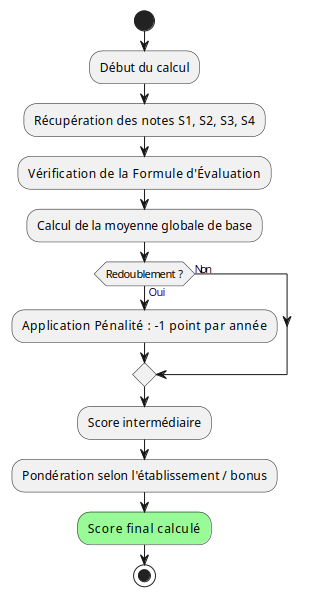
\includegraphics[width=2.97361in,height=6.12569in]{media/image13.png}
\end{itemize}

\subsection{Bonus de mention et coefficient
diplôme}

Le score brut est enrichi par deux mécanismes de bonification :

\begin{longtable}[]{@{}
  >{\raggedright\arraybackslash}p{(\columnwidth - 2\tabcolsep) * \real{0.4865}}
  >{\raggedright\arraybackslash}p{(\columnwidth - 2\tabcolsep) * \real{0.4865}}@{}}
\toprule\noalign{}
\begin{minipage}[b]{\linewidth}\raggedright
\textbf{Mention}
\end{minipage} & \begin{minipage}[b]{\linewidth}\raggedright
\textbf{Bonus}
\end{minipage} \\
\midrule\noalign{}
\endhead
\bottomrule\noalign{}
\endlastfoot
Très Bien ($\geq$ 16) & +2.0 points \\
Bien ($\geq$ 14) & +1.5 points \\
Assez Bien ($\geq$ 12) & +1.0 point \\
Passable ($\geq$ 10) & +0.0 point \\
\end{longtable}

Un coefficient multiplicateur est appliqué selon le type de diplôme :

\begin{longtable}[]{@{}
  >{\raggedright\arraybackslash}p{(\columnwidth - 2\tabcolsep) * \real{0.4865}}
  >{\raggedright\arraybackslash}p{(\columnwidth - 2\tabcolsep) * \real{0.4865}}@{}}
\toprule\noalign{}
\begin{minipage}[b]{\linewidth}\raggedright
\textbf{Type de diplôme}
\end{minipage} & \begin{minipage}[b]{\linewidth}\raggedright
\textbf{Coefficient}
\end{minipage} \\
\midrule\noalign{}
\endhead
\bottomrule\noalign{}
\endlastfoot
DUT / BTS (spécialité correspondante) & ×1.00 \\
Licence (spécialité correspondante) & ×1.00 \\
Autre diplôme reconnu & ×0.80 \\
\end{longtable}

\subsection{Formule du score final}

Le score final intègre la note de l\textquotesingle épreuve écrite selon
la formule :

\textbf{Score\_final = (Score\_dossier × 0.40) +
(Note\_épreuve\_normalisée × 0.60)}

En cas d\textquotesingle égalité de score final, le départage se fait
par : (1) la note d\textquotesingle épreuve écrite, (2) la moyenne
générale du dossier, (3) la date de soumission.

\section{Pipeline OCR et Fuzzy
Matching}

\subsection{Extraction OCR}

Le pipeline de traitement automatique des relevés de notes
s\textquotesingle appuie sur les bibliothèques pdfplumber (pour les PDF
natifs) et pytesseract (pour les documents scannés). Le texte brut est
extrait puis soumis à un processus de nettoyage.

\begin{figure}[htbp]
\centering
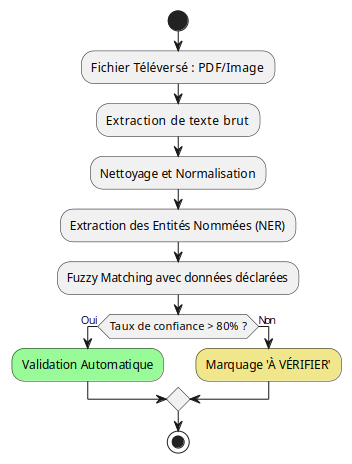
\includegraphics[width=2.71319in,height=4.03056in]{media/image15.png}
\end{figure}

\subsection{Nettoyage du bruit OCR}

Une fonction spécialisée filtre les erreurs fréquentes
d\textquotesingle OCR sur les chiffres et les caractères :

\begin{longtable}[]{@{}
  >{\raggedright\arraybackslash}p{(\columnwidth - 2\tabcolsep) * \real{0.4865}}
  >{\raggedright\arraybackslash}p{(\columnwidth - 2\tabcolsep) * \real{0.4865}}@{}}
\toprule\noalign{}
\caption{Corrections automatiques du bruit OCR} \\
\begin{minipage}[b]{\linewidth}\raggedright
\textbf{Caractère OCR}
\end{minipage} & \begin{minipage}[b]{\linewidth}\raggedright
\textbf{Correction}
\end{minipage} \\
\midrule\noalign{}
\endfirsthead
\caption[]{Corrections automatiques du bruit OCR (suite)} \\
\begin{minipage}[b]{\linewidth}\raggedright
\textbf{Caractère OCR}
\end{minipage} & \begin{minipage}[b]{\linewidth}\raggedright
\textbf{Correction}
\end{minipage} \\
\midrule\noalign{}
\endhead
\bottomrule\noalign{}
\endlastfoot
O (lettre) & 0 (chiffre) \\
l (lettre L min) & 1 (chiffre) \\
S (lettre) & 5 (chiffre) \\
I (lettre I maj) & 1 (chiffre) \\
\end{longtable}

Les textes sont également normalisés : suppression des accents, passage
en minuscules, suppression des caractères spéciaux.

\subsection{Fuzzy Matching des
matières}

L\textquotesingle algorithme utilise la bibliothèque fuzzywuzzy pour
comparer les noms de matières extraits par OCR avec un dictionnaire de
catégories standardisées. Le processus :

\begin{itemize}
\item
  Chaque nom de matière extrait est comparé à toutes les entrées du
  dictionnaire
\item
  La fonction fuzz.token\_sort\_ratio calcule un score de similarité
  entre 0 et 100
\item
  Un seuil strict de 80\% est appliqué : seules les correspondances
  au-dessus sont retenues
\item
  Les catégories standardisées sont : MATH, INFO, CHIMIE\_BIO,
  ELEC\_AUTO, RESEAUX\_BD, LANGUES
\end{itemize}

Exemple : "Mathématiques pour l\textquotesingle ingénieur" → MATH
(similarité 92\%)

Exemple : "Algorithmique et structures de données" → INFO (similarité
85\%)

\subsection{Scoring avec fallback}

Les notes extraites sont regroupées par catégorie standardisée. Si une
catégorie indispensable à la filière n\textquotesingle est pas détectée
par le fuzzy matching, le moteur applique la moyenne générale du
candidat comme valeur de remplacement (fallback) et marque
automatiquement le dossier comme SUSPECT pour vérification manuelle par
le responsable.

\section{Calcul automatique des
mentions}

La mention est calculée automatiquement dans la méthode save() du modèle
NoteSemestre. La validation stricte impose que les moyennes soient dans
la plage {[}10.00, 20.00{]}. Toute valeur hors plage déclenche une
ValidationError Django.

Le champ mention est déclaré avec editable=False pour empêcher toute
modification manuelle. Il est recalculé à chaque sauvegarde selon les
seuils LMD définis précédemment dans la section 1.3.3.

\section{Conclusion}

Ce chapitre a présenté les algorithmes au cœur de la plateforme : le
moteur de règles de rejet à 7 types, le scoring pondéré par filière avec
ses formules mathématiques, et le pipeline OCR avec fuzzy matching. Ces
mécanismes garantissent un traitement automatisé, fiable et transparent
des candidatures. Le chapitre suivant détaillera
l\textquotesingle implémentation, la gestion de
l\textquotesingle asynchronisme et les tests.

\chapter{Implémentation, Asynchronisme et
Tests}

\section{Introduction}

Ce chapitre présente les aspects concrets de
l\textquotesingle implémentation : les interfaces développées, la
gestion de l\textquotesingle asynchronisme pour les opérations
coûteuses, le système de notifications en temps réel, la sécurité et la
stratégie de tests.

\section{Interfaces
développées}

L\textquotesingle application comprend 11 interfaces principales,
couvrant les trois rôles d\textquotesingle utilisateurs (Candidat,
Responsable, Administrateur) :

\begin{longtable}[]{@{}
  >{\raggedright\arraybackslash}p{(\columnwidth - 4\tabcolsep) * \real{0.3243}}
  >{\raggedright\arraybackslash}p{(\columnwidth - 4\tabcolsep) * \real{0.3243}}
  >{\raggedright\arraybackslash}p{(\columnwidth - 4\tabcolsep) * \real{0.3243}}@{}}
\toprule\noalign{}
\caption{Interfaces développées par rôle} \\
\begin{minipage}[b]{\linewidth}\raggedright
\textbf{Interface}
\end{minipage} & \begin{minipage}[b]{\linewidth}\raggedright
\textbf{Rôle}
\end{minipage} & \begin{minipage}[b]{\linewidth}\raggedright
\textbf{Description}
\end{minipage} \\
\midrule\noalign{}
\endfirsthead
\caption[]{Interfaces développées par rôle (suite)} \\
\begin{minipage}[b]{\linewidth}\raggedright
\textbf{Interface}
\end{minipage} & \begin{minipage}[b]{\linewidth}\raggedright
\textbf{Rôle}
\end{minipage} & \begin{minipage}[b]{\linewidth}\raggedright
\textbf{Description}
\end{minipage} \\
\midrule\noalign{}
\endhead
\bottomrule\noalign{}
\endlastfoot
Page d\textquotesingle accueil & Public & Landing page avec statistiques
ENSA BM et filières \\
Authentification & Public & Inscription (email + CIN) et connexion
JWT \\
Formulaire candidature & Candidat & 5 étapes avec sauvegarde
brouillon \\
Suivi de dossier & Candidat & Statut temps réel avec badges colorés \\
Résultats épreuve & Candidat & Note, rang et résultat (Admis/Recalé) \\
Dashboard responsable & Responsable & KPIs, graphiques Recharts,
actions \\
Gestion des dossiers & Responsable & Liste paginée, filtres, tri par
score \\
Détail dossier & Responsable & Vue complète avec historique et
alertes \\
Configuration admin & Admin & Filières, règles, pondérations \\
Import Excel & Responsable & Wizard 3 étapes avec mapping colonnes \\
Notifications & Tous & Cloche, panneau déroulant, historique \\
\end{longtable}

\begin{figure}[htbp]
\centering

\includegraphics[width=6.33472in,height=2.97917in]{media/image17.png}
\end{figure}

\section{}

\begin{figure}[htbp]
\centering
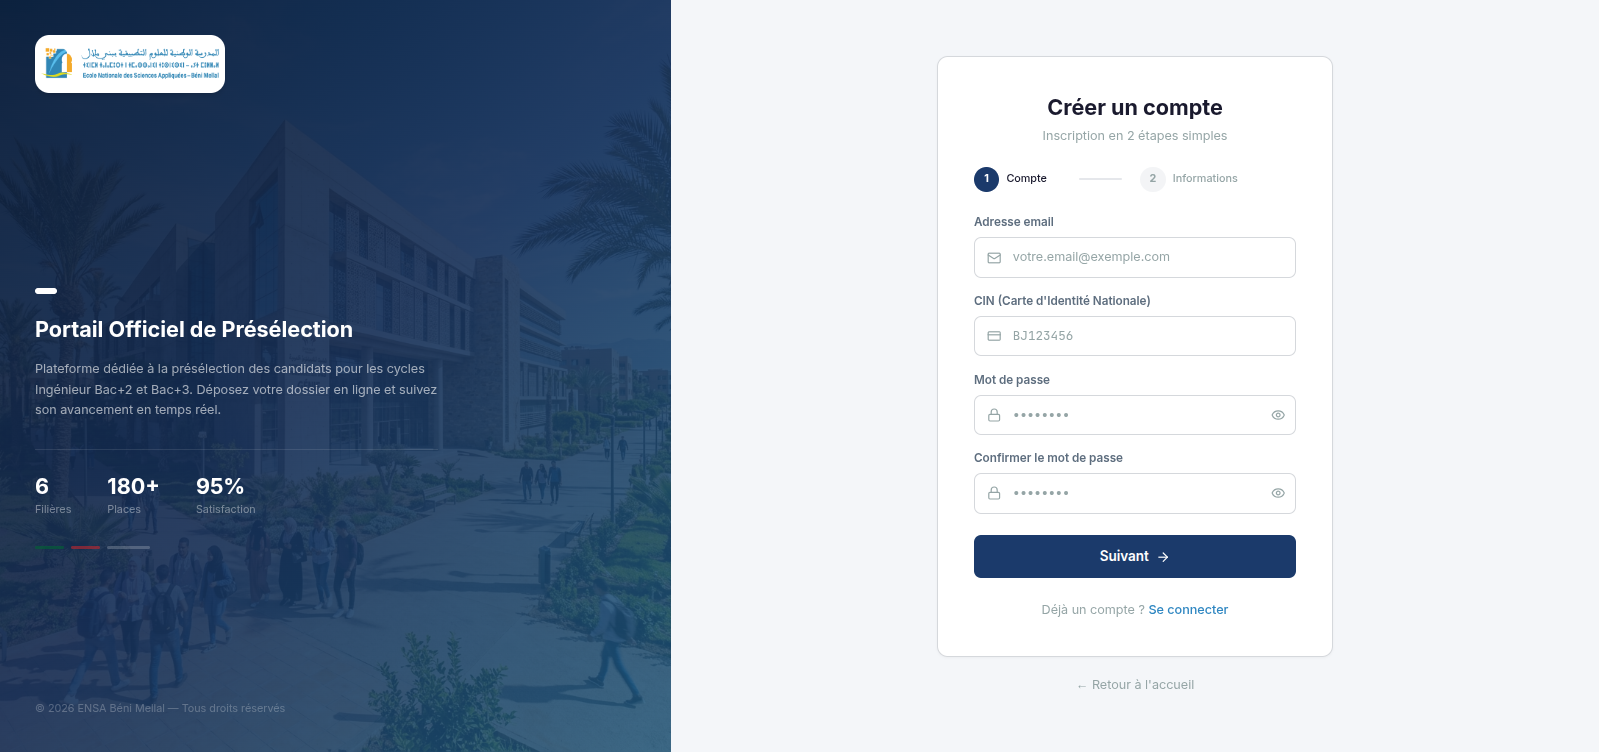
\includegraphics[width=6.33472in,height=2.97917in]{media/image18.png}
\end{figure}

\section{}

\begin{figure}[htbp]
\centering
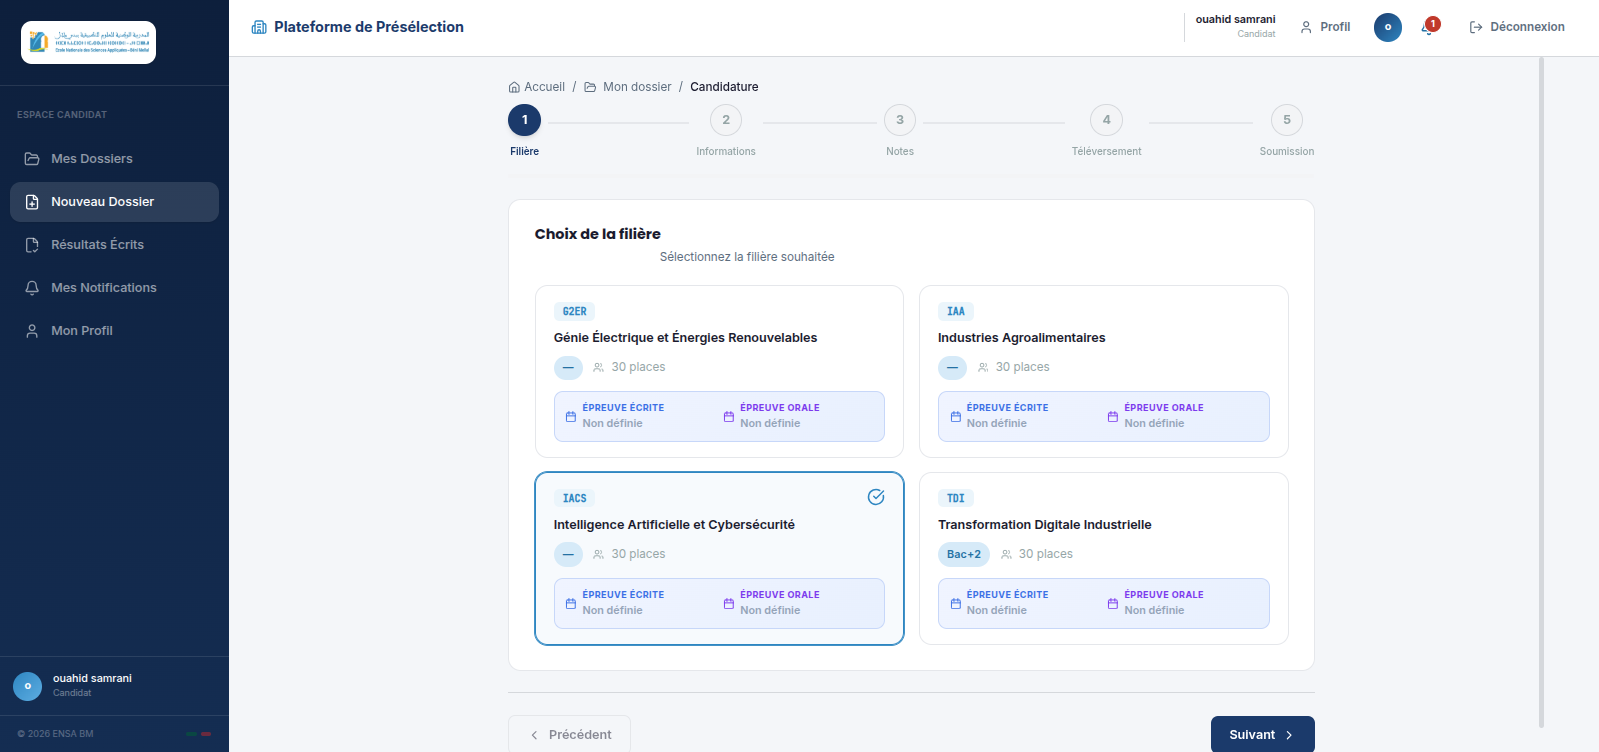
\includegraphics[width=6.33472in,height=2.97917in]{media/image19.png}
\end{figure}


\section{\texorpdfstring{\protect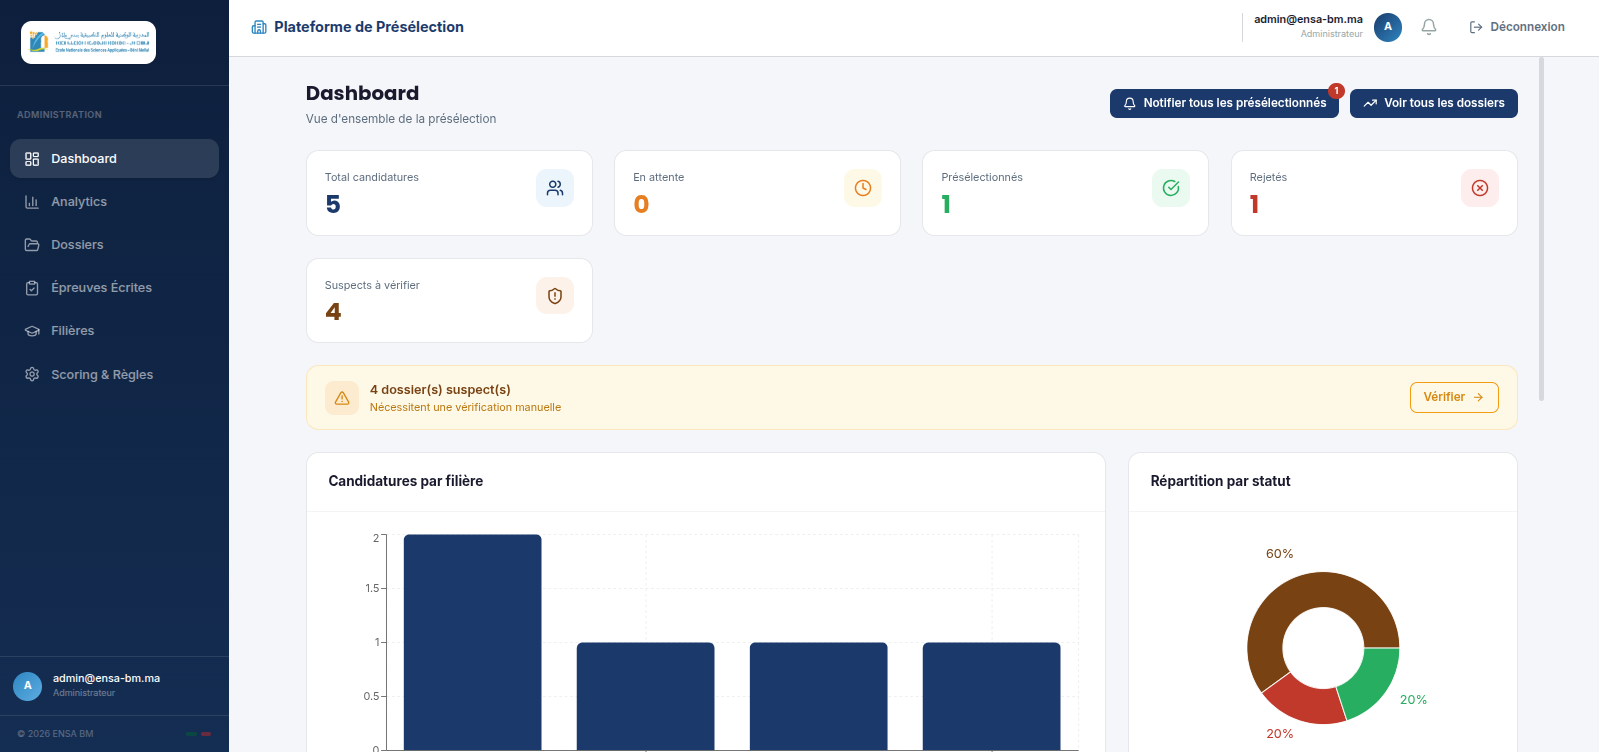
\includegraphics[width=6.33472in,height=2.97917in]{media/image20.png}}{}}


\section{\texorpdfstring{\protect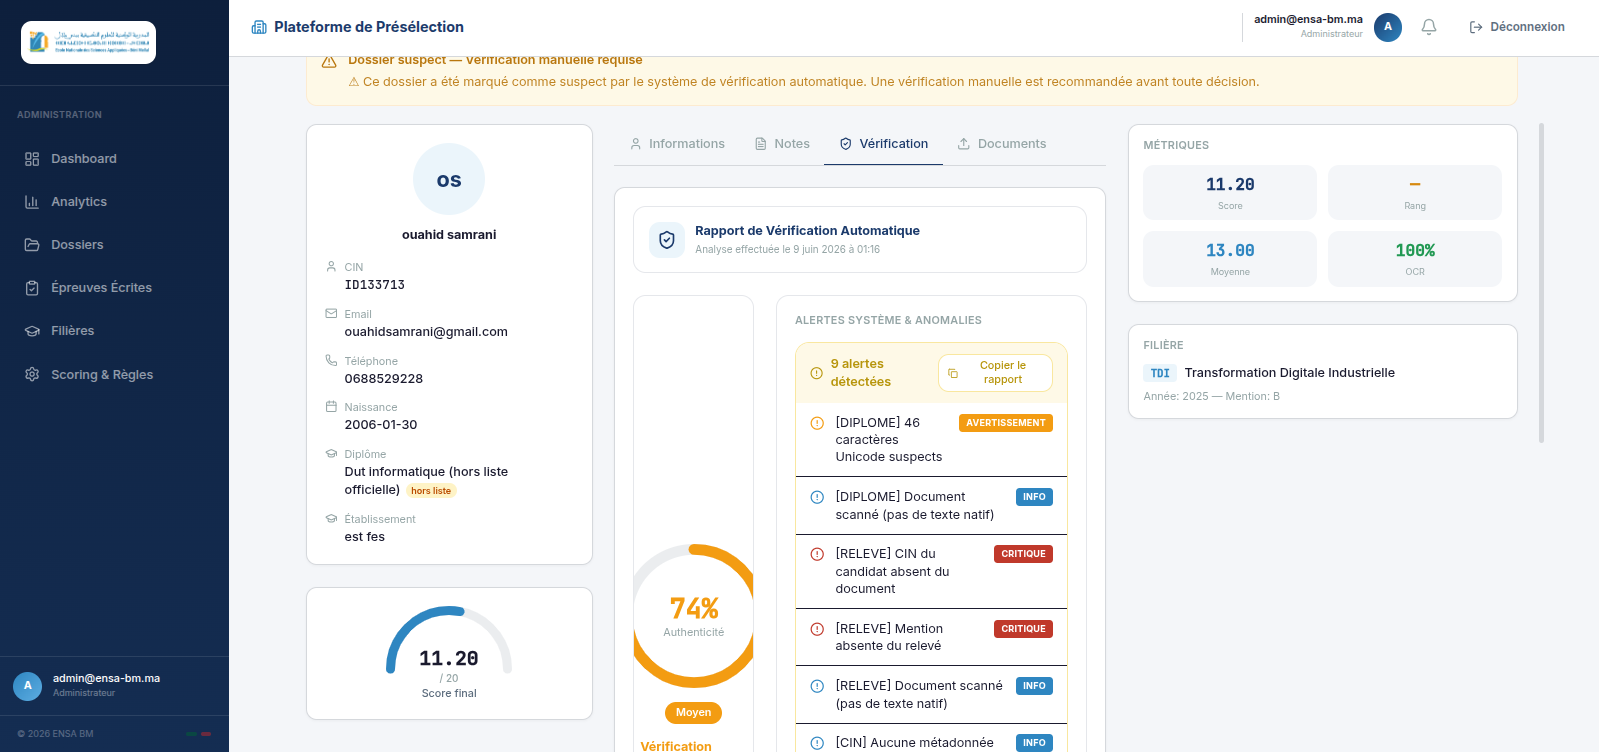
\includegraphics[width=6.33472in,height=2.97917in]{media/image21.png}}{}}


\section{\texorpdfstring{\protect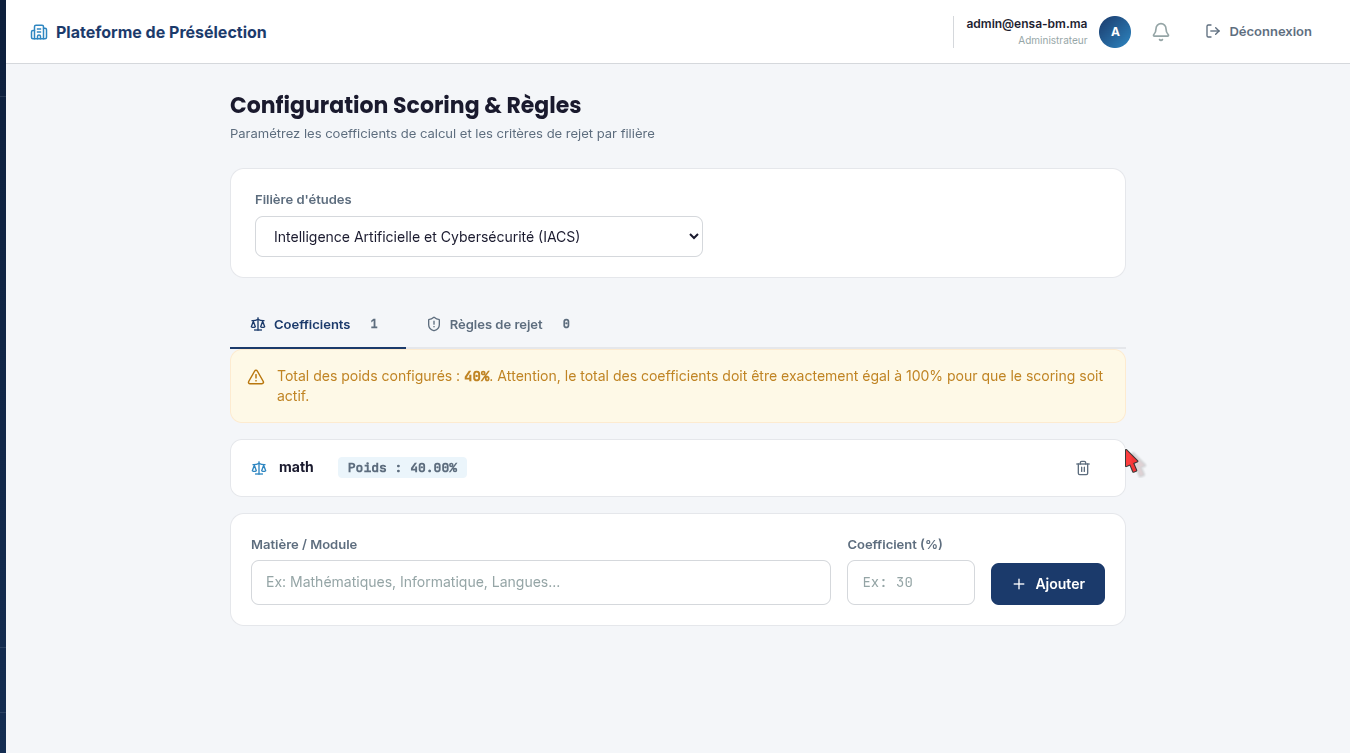
\includegraphics[width=6.33472in,height=3.53333in]{media/image22.png}}{}}


\section{\texorpdfstring{\protect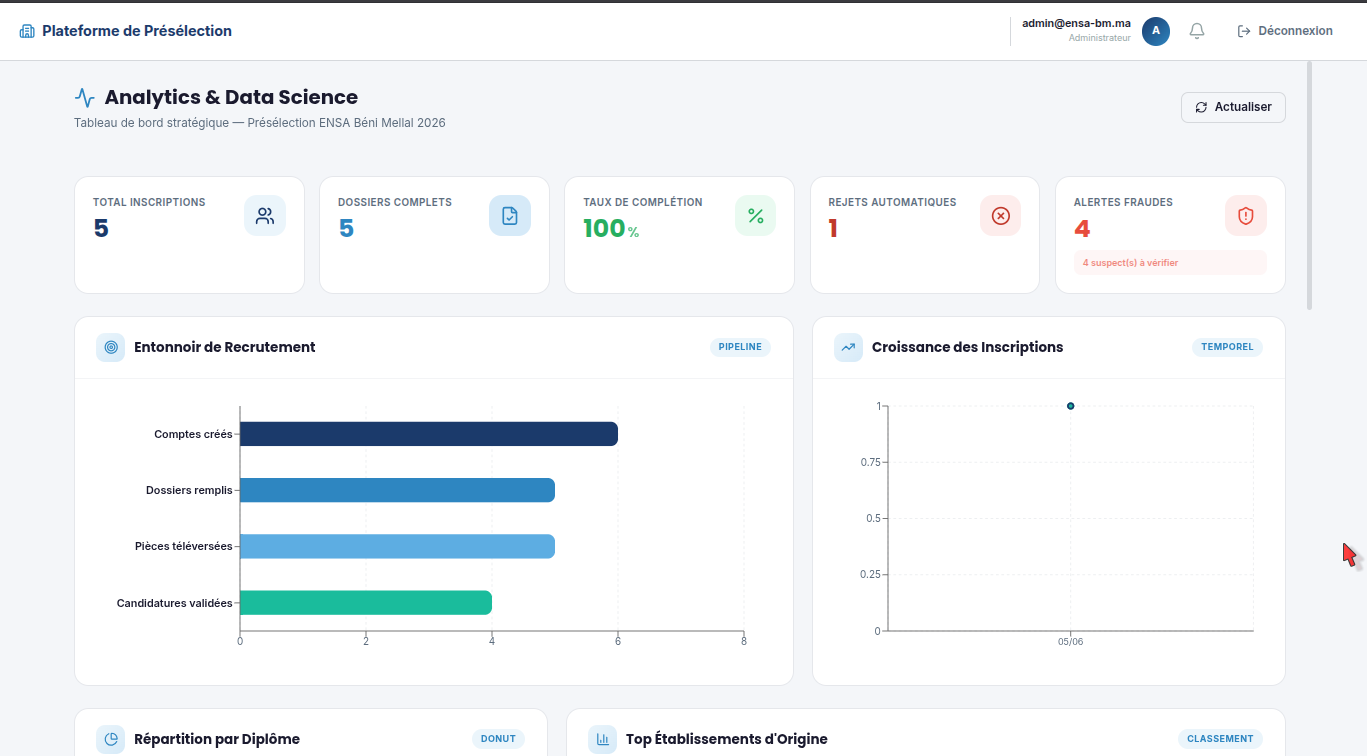
\includegraphics[width=6.33472in,height=3.50278in]{media/image23.png}}{}}

\section{Gestion de
l\textquotesingle asynchronisme}

\subsection{Problématique}

Plusieurs opérations de la plateforme sont coûteuses en temps
d\textquotesingle exécution : le traitement OCR des documents, le calcul
des scores, l\textquotesingle envoi d\textquotesingle emails en masse.
Un traitement synchrone bloquerait l\textquotesingle interface
utilisateur pendant plusieurs secondes.

\subsection{Solution :
threading.Thread}

Pour garantir une excellente expérience utilisateur,
l\textquotesingle application utilise l\textquotesingle asynchronisme
via threading.Thread de Python. Les processus lourds sont exécutés en
arrière-plan dans des threads démons. Le flux est le suivant :

\begin{itemize}
\item
  Le candidat soumet son dossier → réponse HTTP 200 immédiate
\item
  Un thread démon est lancé pour le traitement OCR et le scoring
\item
  Le thread ferme correctement sa connexion à la base de données après
  exécution
\item
  Le candidat est redirigé instantanément vers son dashboard
\item
  Le statut du dossier est mis à jour en arrière-plan et notifié via
  WebSocket
\end{itemize}

\subsection{Gestion des connexions base de
données}

Le système veille à clore correctement les connexions à la base de
données dans les threads via django.db.connections.close\_all() pour
éviter toute fuite de connexion ou conflit d\textquotesingle accès
concurrent.

\section{Système de notifications en temps
réel}

\subsection{Architecture WebSocket}

Les notifications combinent deux canaux complémentaires :

\begin{itemize}
\item
  SMTP (Gmail App Password) : envoi d\textquotesingle emails avec
  gestion des erreurs et statut persisté
\item
  Django Channels + Redis : notifications WebSocket temps réel avec
  barre de progression pour les envois en masse
\end{itemize}

\subsection{Envoi en masse avec
progression}

Lors de l\textquotesingle envoi de notifications en masse, le backend
envoie les emails par batch SMTP et notifie le frontend de la
progression en temps réel via WebSocket. Le responsable voit une barre
de progression se remplir au fur et à mesure des envois.

\section{Système de logging}

L\textquotesingle application intègre un mécanisme de traçabilité
sécurisé par fichiers. La configuration Django dirige les flux vers un
fichier central (logs/ensa\_presel.log). Les logs sont structurés par
domaine :

\begin{longtable}[]{@{}
  >{\raggedright\arraybackslash}p{(\columnwidth - 4\tabcolsep) * \real{0.3243}}
  >{\raggedright\arraybackslash}p{(\columnwidth - 4\tabcolsep) * \real{0.3243}}
  >{\raggedright\arraybackslash}p{(\columnwidth - 4\tabcolsep) * \real{0.3243}}@{}}
\toprule\noalign{}
\caption{Configuration des loggers} \\
\begin{minipage}[b]{\linewidth}\raggedright
\textbf{Logger}
\end{minipage} & \begin{minipage}[b]{\linewidth}\raggedright
\textbf{Niveau}
\end{minipage} & \begin{minipage}[b]{\linewidth}\raggedright
\textbf{Usage}
\end{minipage} \\
\midrule\noalign{}
\endfirsthead
\caption[]{Configuration des loggers (suite)} \\
\begin{minipage}[b]{\linewidth}\raggedright
\textbf{Logger}
\end{minipage} & \begin{minipage}[b]{\linewidth}\raggedright
\textbf{Niveau}
\end{minipage} & \begin{minipage}[b]{\linewidth}\raggedright
\textbf{Usage}
\end{minipage} \\
\midrule\noalign{}
\endhead
\bottomrule\noalign{}
\endlastfoot
django & WARNING & Erreurs framework \\
candidatures & INFO & Opérations métier \\
notifications & INFO & Envois email/WebSocket \\
channels & DEBUG & Connexions WebSocket \\
\end{longtable}

\section{Sécurité de
l\textquotesingle application}

\begin{longtable}[]{@{}
  >{\raggedright\arraybackslash}p{(\columnwidth - 2\tabcolsep) * \real{0.4865}}
  >{\raggedright\arraybackslash}p{(\columnwidth - 2\tabcolsep) * \real{0.4865}}@{}}
\toprule\noalign{}
\caption{Mesures de sécurité implémentées} \\
\begin{minipage}[b]{\linewidth}\raggedright
\textbf{Mesure}
\end{minipage} & \begin{minipage}[b]{\linewidth}\raggedright
\textbf{Implémentation}
\end{minipage} \\
\midrule\noalign{}
\endfirsthead
\caption[]{Mesures de sécurité implémentées (suite)} \\
\begin{minipage}[b]{\linewidth}\raggedright
\textbf{Mesure}
\end{minipage} & \begin{minipage}[b]{\linewidth}\raggedright
\textbf{Implémentation}
\end{minipage} \\
\midrule\noalign{}
\endhead
\bottomrule\noalign{}
\endlastfoot
Authentification & JWT (access 15min + refresh 24h) \\
Autorisation & RBAC à 3 niveaux via @permission\_classes \\
CSRF & Protection Django middleware activée \\
XSS & Échappement automatique Django + React \\
Injection SQL & ORM Django avec requêtes paramétrées \\
Logs sécurisés & Fichier avec rotation, pas de console \\
Confidentialité & Scores OCR masqués côté candidat \\
\end{longtable}

\section{Stratégie de tests}

\subsection{Niveaux de tests}

\begin{longtable}[]{@{}
  >{\raggedright\arraybackslash}p{(\columnwidth - 4\tabcolsep) * \real{0.3243}}
  >{\raggedright\arraybackslash}p{(\columnwidth - 4\tabcolsep) * \real{0.3243}}
  >{\raggedright\arraybackslash}p{(\columnwidth - 4\tabcolsep) * \real{0.3243}}@{}}
\toprule\noalign{}
\begin{minipage}[b]{\linewidth}\raggedright
\textbf{Niveau}
\end{minipage} & \begin{minipage}[b]{\linewidth}\raggedright
\textbf{Objectif}
\end{minipage} & \begin{minipage}[b]{\linewidth}\raggedright
\textbf{Outils}
\end{minipage} \\
\midrule\noalign{}
\endhead
\bottomrule\noalign{}
\endlastfoot
Tests unitaires & Valider chaque composant isolément & Django
TestCase \\
Tests d\textquotesingle intégration & Valider les flux complets &
APITestCase, APIClient \\
Tests fonctionnels & Valider les scénarios utilisateur & Scénarios
manuels \\
Tests d\textquotesingle interface & Valider le responsive et
l\textquotesingle UX & Navigateur, DevTools \\
\end{longtable}

\subsection{Tests du moteur de
règles}

\begin{longtable}[]{@{}
  >{\raggedright\arraybackslash}p{(\columnwidth - 6\tabcolsep) * \real{0.2432}}
  >{\raggedright\arraybackslash}p{(\columnwidth - 6\tabcolsep) * \real{0.2432}}
  >{\raggedright\arraybackslash}p{(\columnwidth - 6\tabcolsep) * \real{0.2432}}
  >{\raggedright\arraybackslash}p{(\columnwidth - 6\tabcolsep) * \real{0.2432}}@{}}
\toprule\noalign{}
\begin{minipage}[b]{\linewidth}\raggedright
\textbf{Test}
\end{minipage} & \begin{minipage}[b]{\linewidth}\raggedright
\textbf{Entrée}
\end{minipage} & \begin{minipage}[b]{\linewidth}\raggedright
\textbf{Résultat attendu}
\end{minipage} & \begin{minipage}[b]{\linewidth}\raggedright
\textbf{Statut}
\end{minipage} \\
\midrule\noalign{}
\endhead
\bottomrule\noalign{}
\endlastfoot
Diplôme invalide & DUT non accepté pour TDI & REJETE\_AUTO & $\checkmark$ Passé \\
Moyenne insuffisante & Moyenne 9.5 (seuil 10) & REJETE\_AUTO & $\checkmark$
Passé \\
Doublon CIN & CIN déjà existant & REJETE\_AUTO & $\checkmark$ Passé \\
Dossier conforme & Tous critères OK & EN\_ATTENTE & $\checkmark$ Passé \\
\end{longtable}

\subsection{Tests de l\textquotesingle algorithme de
scoring}

\begin{longtable}[]{@{}
  >{\raggedright\arraybackslash}p{(\columnwidth - 6\tabcolsep) * \real{0.2432}}
  >{\raggedright\arraybackslash}p{(\columnwidth - 6\tabcolsep) * \real{0.2432}}
  >{\raggedright\arraybackslash}p{(\columnwidth - 6\tabcolsep) * \real{0.2432}}
  >{\raggedright\arraybackslash}p{(\columnwidth - 6\tabcolsep) * \real{0.2432}}@{}}
\toprule\noalign{}
\begin{minipage}[b]{\linewidth}\raggedright
\textbf{Test}
\end{minipage} & \begin{minipage}[b]{\linewidth}\raggedright
\textbf{Données}
\end{minipage} & \begin{minipage}[b]{\linewidth}\raggedright
\textbf{Score attendu}
\end{minipage} & \begin{minipage}[b]{\linewidth}\raggedright
\textbf{Statut}
\end{minipage} \\
\midrule\noalign{}
\endhead
\bottomrule\noalign{}
\endlastfoot
Scoring TDI & Moyennes S1-S6, DUT Info & 15.42 & $\checkmark$ Passé \\
Scoring IACS & Moyennes S1-S6, Licence Info & 14.87 & $\checkmark$ Passé \\
Bonus mention TB & Moyenne $\geq$16 & +2.0 bonus & $\checkmark$ Passé \\
\end{longtable}

\subsection{Récapitulatif des
tests}

\begin{longtable}[]{@{}
  >{\raggedright\arraybackslash}p{(\columnwidth - 6\tabcolsep) * \real{0.2432}}
  >{\raggedright\arraybackslash}p{(\columnwidth - 6\tabcolsep) * \real{0.2432}}
  >{\raggedright\arraybackslash}p{(\columnwidth - 6\tabcolsep) * \real{0.2432}}
  >{\raggedright\arraybackslash}p{(\columnwidth - 6\tabcolsep) * \real{0.2432}}@{}}
\toprule\noalign{}
\begin{minipage}[b]{\linewidth}\raggedright
\textbf{Type de test}
\end{minipage} & \begin{minipage}[b]{\linewidth}\raggedright
\textbf{Nombre}
\end{minipage} & \begin{minipage}[b]{\linewidth}\raggedright
\textbf{Passés}
\end{minipage} & \begin{minipage}[b]{\linewidth}\raggedright
\textbf{Échoués}
\end{minipage} \\
\midrule\noalign{}
\endhead
\bottomrule\noalign{}
\endlastfoot
Unitaires & 32 & 32 & 0 \\
Intégration & 12 & 12 & 0 \\
Fonctionnels & 9 & 9 & 0 \\
Interface & 8 & 8 & 0 \\
Total & 61 & 61 & 0 \\
\end{longtable}

\emph{Tableau 4.4 : Récapitulatif des résultats de tests}

\subsection{Couverture de code}

\begin{longtable}[]{@{}
  >{\raggedright\arraybackslash}p{(\columnwidth - 2\tabcolsep) * \real{0.4865}}
  >{\raggedright\arraybackslash}p{(\columnwidth - 2\tabcolsep) * \real{0.4865}}@{}}
\toprule\noalign{}
\begin{minipage}[b]{\linewidth}\raggedright
\textbf{Module}
\end{minipage} & \begin{minipage}[b]{\linewidth}\raggedright
\textbf{Couverture}
\end{minipage} \\
\midrule\noalign{}
\endhead
\bottomrule\noalign{}
\endlastfoot
users & 89\% \\
candidatures & 92\% \\
administration & 85\% \\
scoring & 94\% \\
notifications & 78\% \\
Global & 87\% \\
\end{longtable}

\section{Difficultés rencontrées et
solutions}

\begin{longtable}[]{@{}
  >{\raggedright\arraybackslash}p{(\columnwidth - 2\tabcolsep) * \real{0.4865}}
  >{\raggedright\arraybackslash}p{(\columnwidth - 2\tabcolsep) * \real{0.4865}}@{}}
\toprule\noalign{}
\caption{Difficultés rencontrées et solutions} \\
\begin{minipage}[b]{\linewidth}\raggedright
\textbf{Difficulté}
\end{minipage} & \begin{minipage}[b]{\linewidth}\raggedright
\textbf{Solution apportée}
\end{minipage} \\
\midrule\noalign{}
\endfirsthead
\caption[]{Difficultés rencontrées et solutions (suite)} \\
\begin{minipage}[b]{\linewidth}\raggedright
\textbf{Difficulté}
\end{minipage} & \begin{minipage}[b]{\linewidth}\raggedright
\textbf{Solution apportée}
\end{minipage} \\
\midrule\noalign{}
\endhead
\bottomrule\noalign{}
\endlastfoot
WebSocket + JWT expiré & Middleware WebSocket avec refresh automatique
du token \\
SMTP Gmail bloqué & Configuration App Password avec gestion des
erreurs \\
Imports circulaires Django & Import local dans les méthodes au lieu
d\textquotesingle imports globaux \\
OCR faible qualité & Fallback sur moyenne générale + flag SUSPECT \\
Connexions DB dans threads & Appel systématique à
connections.close\_all() \\
\end{longtable}

\section{Conclusion}

Ce chapitre a présenté les aspects concrets de
l\textquotesingle implémentation : les 11 interfaces développées, la
gestion de l\textquotesingle asynchronisme via threading, le système de
notifications WebSocket temps réel, la sécurité robuste et la stratégie
de tests complète avec un taux de réussite de 100\% et une couverture de
code de 87\%.
